\documentclass[twoside]{book}

% Packages required by doxygen
\usepackage{fixltx2e}
\usepackage{calc}
\usepackage{doxygen}
\usepackage[export]{adjustbox} % also loads graphicx
\usepackage{graphicx}
\usepackage[utf8]{inputenc}
\usepackage{makeidx}
\usepackage{multicol}
\usepackage{multirow}
\PassOptionsToPackage{warn}{textcomp}
\usepackage{textcomp}
\usepackage[nointegrals]{wasysym}
\usepackage[table]{xcolor}

% Font selection
\usepackage[T1]{fontenc}
\usepackage[scaled=.90]{helvet}
\usepackage{courier}
\usepackage{amssymb}
\usepackage{sectsty}
\renewcommand{\familydefault}{\sfdefault}
\allsectionsfont{%
  \fontseries{bc}\selectfont%
  \color{darkgray}%
}
\renewcommand{\DoxyLabelFont}{%
  \fontseries{bc}\selectfont%
  \color{darkgray}%
}
\newcommand{\+}{\discretionary{\mbox{\scriptsize$\hookleftarrow$}}{}{}}

% Page & text layout
\usepackage{geometry}
\geometry{%
  a4paper,%
  top=2.5cm,%
  bottom=2.5cm,%
  left=2.5cm,%
  right=2.5cm%
}
\tolerance=750
\hfuzz=15pt
\hbadness=750
\setlength{\emergencystretch}{15pt}
\setlength{\parindent}{0cm}
\setlength{\parskip}{3ex plus 2ex minus 2ex}
\makeatletter
\renewcommand{\paragraph}{%
  \@startsection{paragraph}{4}{0ex}{-1.0ex}{1.0ex}{%
    \normalfont\normalsize\bfseries\SS@parafont%
  }%
}
\renewcommand{\subparagraph}{%
  \@startsection{subparagraph}{5}{0ex}{-1.0ex}{1.0ex}{%
    \normalfont\normalsize\bfseries\SS@subparafont%
  }%
}
\makeatother

% Headers & footers
\usepackage{fancyhdr}
\pagestyle{fancyplain}
\fancyhead[LE]{\fancyplain{}{\bfseries\thepage}}
\fancyhead[CE]{\fancyplain{}{}}
\fancyhead[RE]{\fancyplain{}{\bfseries\leftmark}}
\fancyhead[LO]{\fancyplain{}{\bfseries\rightmark}}
\fancyhead[CO]{\fancyplain{}{}}
\fancyhead[RO]{\fancyplain{}{\bfseries\thepage}}
\fancyfoot[LE]{\fancyplain{}{}}
\fancyfoot[CE]{\fancyplain{}{}}
\fancyfoot[RE]{\fancyplain{}{\bfseries\scriptsize Generated by Doxygen }}
\fancyfoot[LO]{\fancyplain{}{\bfseries\scriptsize Generated by Doxygen }}
\fancyfoot[CO]{\fancyplain{}{}}
\fancyfoot[RO]{\fancyplain{}{}}
\renewcommand{\footrulewidth}{0.4pt}
\renewcommand{\chaptermark}[1]{%
  \markboth{#1}{}%
}
\renewcommand{\sectionmark}[1]{%
  \markright{\thesection\ #1}%
}

% Indices & bibliography
\usepackage{natbib}
\usepackage[titles]{tocloft}
\setcounter{tocdepth}{3}
\setcounter{secnumdepth}{5}
\makeindex

% Hyperlinks (required, but should be loaded last)
\usepackage{ifpdf}
\ifpdf
  \usepackage[pdftex,pagebackref=true]{hyperref}
\else
  \usepackage[ps2pdf,pagebackref=true]{hyperref}
\fi
\hypersetup{%
  colorlinks=true,%
  linkcolor=blue,%
  citecolor=blue,%
  unicode%
}

% Custom commands
\newcommand{\clearemptydoublepage}{%
  \newpage{\pagestyle{empty}\cleardoublepage}%
}

\usepackage{caption}
\captionsetup{labelsep=space,justification=centering,font={bf},singlelinecheck=off,skip=4pt,position=top}

%===== C O N T E N T S =====

\begin{document}

% Titlepage & ToC
\hypersetup{pageanchor=false,
             bookmarksnumbered=true,
             pdfencoding=unicode
            }
\pagenumbering{alph}
\begin{titlepage}
\vspace*{7cm}
\begin{center}%
{\Large Cage\+Control \\[1ex]\large Control waveplates inside tomography cages }\\
\vspace*{1cm}
{\large Generated by Doxygen 1.8.13}\\
\end{center}
\end{titlepage}
\clearemptydoublepage
\pagenumbering{roman}
\tableofcontents
\clearemptydoublepage
\pagenumbering{arabic}
\hypersetup{pageanchor=true}

%--- Begin generated contents ---
\chapter{Bug List}
\label{bug}
\Hypertarget{bug}

\begin{DoxyRefList}
\item[\label{bug__bug000001}%
\Hypertarget{bug__bug000001}%
File \hyperlink{debug_8h}{debug.h} ]Printing to console does not work on Windows. Workaround\+: Redirect stderr to stdout and redirect stdout to a file. 
\item[\label{bug__bug000002}%
\Hypertarget{bug__bug000002}%
File \hyperlink{defines_8h}{defines.h} ]There are no known bugs. 
\item[\label{bug__bug000003}%
\Hypertarget{bug__bug000003}%
Namespace \hyperlink{namespacehelper}{helper} ]There are no known bugs.  
\item[\label{bug__bug000004}%
\Hypertarget{bug__bug000004}%
Class \hyperlink{classMotor}{Motor} ]There are no known bugs. 
\item[\label{bug__bug000005}%
\Hypertarget{bug__bug000005}%
Class \hyperlink{classUDPlistener}{U\+D\+Plistener} ]There are no known bugs 
\item[\label{bug__bug000006}%
\Hypertarget{bug__bug000006}%
File \hyperlink{version_8h}{version.h} ]There are no known bugs.
\end{DoxyRefList}
\chapter{Namespace Index}
\section{Namespace List}
Here is a list of all documented namespaces with brief descriptions\+:\begin{DoxyCompactList}
\item\contentsline{section}{\hyperlink{namespacehelper}{helper} \\*Small functions to display messages }{\pageref{namespacehelper}}{}
\end{DoxyCompactList}

\chapter{Hierarchical Index}
\section{Class Hierarchy}
This inheritance list is sorted roughly, but not completely, alphabetically\+:\begin{DoxyCompactList}
\item Q\+Main\+Window\begin{DoxyCompactList}
\item \contentsline{section}{cagecontrol}{\pageref{classcagecontrol}}{}
\end{DoxyCompactList}
\item Q\+Object\begin{DoxyCompactList}
\item \contentsline{section}{Motor}{\pageref{classMotor}}{}
\end{DoxyCompactList}
\end{DoxyCompactList}

\chapter{Class Index}
\section{Class List}
Here are the classes, structs, unions and interfaces with brief descriptions\+:\begin{DoxyCompactList}
\item\contentsline{section}{\hyperlink{classcagecontrol}{cagecontrol} }{\pageref{classcagecontrol}}{}
\item\contentsline{section}{\hyperlink{classMotor}{Motor} \\*Operates the P\+C\+B-\/motor }{\pageref{classMotor}}{}
\end{DoxyCompactList}

\chapter{File Index}
\section{File List}
Here is a list of all documented files with brief descriptions\+:\begin{DoxyCompactList}
\item\contentsline{section}{{\bfseries cagecontrol.\+h} }{\pageref{cagecontrol_8h}}{}
\item\contentsline{section}{\hyperlink{debug_8h}{debug.\+h} \\*Debug macros }{\pageref{debug_8h}}{}
\item\contentsline{section}{\hyperlink{defines_8h}{defines.\+h} \\*Various compile-\/time definitions }{\pageref{defines_8h}}{}
\item\contentsline{section}{\hyperlink{helper_8h}{helper.\+h} }{\pageref{helper_8h}}{}
\item\contentsline{section}{\hyperlink{motor_8h}{motor.\+h} }{\pageref{motor_8h}}{}
\item\contentsline{section}{\hyperlink{version_8h}{version.\+h} \\*This file contains information about the code version }{\pageref{version_8h}}{}
\end{DoxyCompactList}

\chapter{Namespace Documentation}
\hypertarget{namespacehelper}{}\section{helper Namespace Reference}
\label{namespacehelper}\index{helper@{helper}}


contains small functions to display messages  


\subsection*{Functions}
\begin{DoxyCompactItemize}
\item 
void \hyperlink{namespacehelper_ab2cc8239d9bf2ae383474c0343205346}{message} (Q\+String msg)
\begin{DoxyCompactList}\small\item\em message displays a message box \end{DoxyCompactList}\item 
void \hyperlink{namespacehelper_a00e308809a0f9d76f3a0ba2ad5f3587c}{error} (Q\+String msg)
\begin{DoxyCompactList}\small\item\em error displays an error-\/messagebox and writes a debug\+\_\+error message to stdout \end{DoxyCompactList}\item 
void \hyperlink{namespacehelper_ac717f710dcb45bf31fba9071ea4fb45f}{warning} (Q\+String msg)
\begin{DoxyCompactList}\small\item\em warning displays warning-\/messagebox and writes a debug\+\_\+warning message to stdout \end{DoxyCompactList}\item 
void \hyperlink{namespacehelper_a88e86d2fd14fc8354c1529beaa157f25}{info} (Q\+String msg)
\begin{DoxyCompactList}\small\item\em info displays an info-\/messagebox and writes a debug\+\_\+info message to stdout \end{DoxyCompactList}\end{DoxyCompactItemize}


\subsection{Detailed Description}
contains small functions to display messages 

\begin{DoxyRefDesc}{Bug}
\item[\hyperlink{bug__bug000003}{Bug}]There are no known bugs. \end{DoxyRefDesc}


\subsection{Function Documentation}
\mbox{\Hypertarget{namespacehelper_a00e308809a0f9d76f3a0ba2ad5f3587c}\label{namespacehelper_a00e308809a0f9d76f3a0ba2ad5f3587c}} 
\index{helper@{helper}!error@{error}}
\index{error@{error}!helper@{helper}}
\subsubsection{\texorpdfstring{error()}{error()}}
{\footnotesize\ttfamily void helper\+::error (\begin{DoxyParamCaption}\item[{Q\+String}]{msg }\end{DoxyParamCaption})}



error displays an error-\/messagebox and writes a debug\+\_\+error message to stdout 


\begin{DoxyParams}{Parameters}
{\em msg} & the message to be displayed \\
\hline
\end{DoxyParams}
\mbox{\Hypertarget{namespacehelper_a88e86d2fd14fc8354c1529beaa157f25}\label{namespacehelper_a88e86d2fd14fc8354c1529beaa157f25}} 
\index{helper@{helper}!info@{info}}
\index{info@{info}!helper@{helper}}
\subsubsection{\texorpdfstring{info()}{info()}}
{\footnotesize\ttfamily void helper\+::info (\begin{DoxyParamCaption}\item[{Q\+String}]{msg }\end{DoxyParamCaption})}



info displays an info-\/messagebox and writes a debug\+\_\+info message to stdout 


\begin{DoxyParams}{Parameters}
{\em msg} & the message to be displayed \\
\hline
\end{DoxyParams}
\mbox{\Hypertarget{namespacehelper_ab2cc8239d9bf2ae383474c0343205346}\label{namespacehelper_ab2cc8239d9bf2ae383474c0343205346}} 
\index{helper@{helper}!message@{message}}
\index{message@{message}!helper@{helper}}
\subsubsection{\texorpdfstring{message()}{message()}}
{\footnotesize\ttfamily void helper\+::message (\begin{DoxyParamCaption}\item[{Q\+String}]{msg }\end{DoxyParamCaption})}



message displays a message box 


\begin{DoxyParams}{Parameters}
{\em msg} & the message to be displayed \\
\hline
\end{DoxyParams}
\mbox{\Hypertarget{namespacehelper_ac717f710dcb45bf31fba9071ea4fb45f}\label{namespacehelper_ac717f710dcb45bf31fba9071ea4fb45f}} 
\index{helper@{helper}!warning@{warning}}
\index{warning@{warning}!helper@{helper}}
\subsubsection{\texorpdfstring{warning()}{warning()}}
{\footnotesize\ttfamily void helper\+::warning (\begin{DoxyParamCaption}\item[{Q\+String}]{msg }\end{DoxyParamCaption})}



warning displays warning-\/messagebox and writes a debug\+\_\+warning message to stdout 


\begin{DoxyParams}{Parameters}
{\em msg} & the message to be displayed \\
\hline
\end{DoxyParams}

\chapter{Class Documentation}
\hypertarget{classcagecontrol}{}\section{cagecontrol Class Reference}
\label{classcagecontrol}\index{cagecontrol@{cagecontrol}}


Inheritance diagram for cagecontrol\+:\nopagebreak
\begin{figure}[H]
\begin{center}
\leavevmode
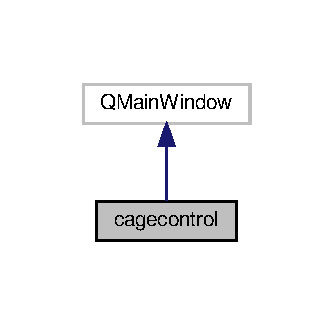
\includegraphics[width=160pt]{classcagecontrol__inherit__graph}
\end{center}
\end{figure}


Collaboration diagram for cagecontrol\+:
\nopagebreak
\begin{figure}[H]
\begin{center}
\leavevmode
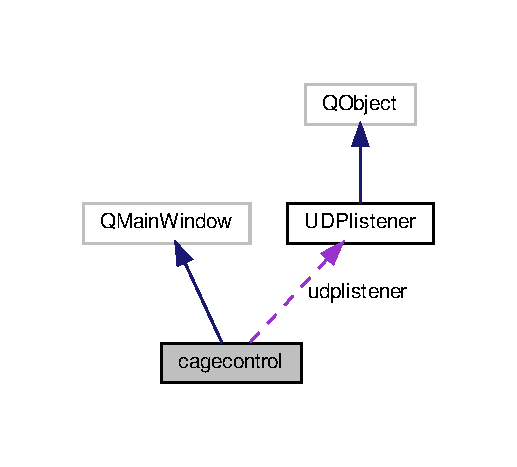
\includegraphics[width=324pt]{classcagecontrol__coll__graph}
\end{center}
\end{figure}
\subsection*{Public Slots}
\begin{DoxyCompactItemize}
\item 
void \hyperlink{classcagecontrol_af9a2772a38394159c54d7e5d7f2a86fb}{slot\+\_\+move\+HV} (Q\+String color)
\begin{DoxyCompactList}\small\item\em move\+HV \end{DoxyCompactList}\item 
void \hyperlink{classcagecontrol_a3207f15cba9458e32fb5c2cf366c4b44}{slot\+\_\+move\+PM} (Q\+String color)
\begin{DoxyCompactList}\small\item\em move\+PM \end{DoxyCompactList}\item 
void \hyperlink{classcagecontrol_a138905383fdc09a0b5077a185eaf6682}{slot\+\_\+move\+LR} (Q\+String color)
\begin{DoxyCompactList}\small\item\em move\+LR \end{DoxyCompactList}\item 
void \hyperlink{classcagecontrol_a2d971435af3267351272b2c2d5f2f709}{slot\+\_\+movemotors} (Q\+String color, double H\+W\+Pang, double Q\+W\+Pang)
\begin{DoxyCompactList}\small\item\em movemotors \end{DoxyCompactList}\end{DoxyCompactItemize}
\subsection*{Public Member Functions}
\begin{DoxyCompactItemize}
\item 
\mbox{\Hypertarget{classcagecontrol_a6630362ef3dd621859126e357e545dd5}\label{classcagecontrol_a6630362ef3dd621859126e357e545dd5}} 
{\bfseries cagecontrol} (Q\+Widget $\ast$parent=nullptr)
\end{DoxyCompactItemize}
\subsection*{Private Slots}
\begin{DoxyCompactItemize}
\item 
void \hyperlink{classcagecontrol_a244c02598b4b73db82b5852561634084}{updatesettings} (double d)
\begin{DoxyCompactList}\small\item\em updatesettings fills variables with data from G\+UI \end{DoxyCompactList}\item 
void \hyperlink{classcagecontrol_a2cfb7b65a7b8838d5f2acaa384a7cfcc}{updatesettingsint} (int i)
\begin{DoxyCompactList}\small\item\em updatesettingsint wrapper, just calls \end{DoxyCompactList}\item 
\mbox{\Hypertarget{classcagecontrol_ab6993b1b41f55c164298c1b3e067ab34}\label{classcagecontrol_ab6993b1b41f55c164298c1b3e067ab34}} 
void \hyperlink{classcagecontrol_ab6993b1b41f55c164298c1b3e067ab34}{update\+UI} ()
\begin{DoxyCompactList}\small\item\em update\+UI updates UI with supposedly new numbers (loaded from conf file, e.\+g.) \end{DoxyCompactList}\end{DoxyCompactItemize}
\subsection*{Private Member Functions}
\begin{DoxyCompactItemize}
\item 
\mbox{\Hypertarget{classcagecontrol_a79a089c4e7196a7c158aa62f4883ba18}\label{classcagecontrol_a79a089c4e7196a7c158aa62f4883ba18}} 
void \hyperlink{classcagecontrol_a79a089c4e7196a7c158aa62f4883ba18}{setup\+UI} (Q\+Grid\+Layout $\ast$layout)
\begin{DoxyCompactList}\small\item\em Puts together the G\+UI. \end{DoxyCompactList}\item 
\mbox{\Hypertarget{classcagecontrol_ae961f42ea421a8d512964f158b0201e8}\label{classcagecontrol_ae961f42ea421a8d512964f158b0201e8}} 
void \hyperlink{classcagecontrol_ae961f42ea421a8d512964f158b0201e8}{openmotors} ()
\begin{DoxyCompactList}\small\item\em Opens serial connections to the P\+CB motor controlllers. \end{DoxyCompactList}\item 
void \hyperlink{classcagecontrol_aab3dedc2c4b814569988c93bd30546c7}{updatestatus} (Q\+String msg)
\begin{DoxyCompactList}\small\item\em updatestatus writes message to statusbar and to a logfile \end{DoxyCompactList}\item 
void \hyperlink{classcagecontrol_a0e6648cef5e6d08d638aa2472824cb6b}{Load\+Config} ()
\begin{DoxyCompactList}\small\item\em Load\+Config loads config from a file. \end{DoxyCompactList}\item 
void \hyperlink{classcagecontrol_a217d948983c0d1c153d29c728b06d764}{Save\+Config} ()
\begin{DoxyCompactList}\small\item\em Save\+Config stores config to a file. \end{DoxyCompactList}\item 
void \hyperlink{classcagecontrol_a2fd60ea2aa138472e3714dbd25cadc55}{motor\+GB} (Q\+Group\+Box $\ast$gb, Q\+String id)
\begin{DoxyCompactList}\small\item\em motor\+GB fills an empty Q\+Group\+Box with motor controls \end{DoxyCompactList}\item 
void \hyperlink{classcagecontrol_a56c01018dbd0d16a360106c438539c9e}{initconnections} ()
\begin{DoxyCompactList}\small\item\em initconnections connects Qt Signals to slots \end{DoxyCompactList}\item 
void \hyperlink{classcagecontrol_a4e2c79dc05f66b2b15ae01eaa8d39fca}{movemotor} (Q\+String motor, double H\+W\+Pang, double Q\+W\+Pang)
\begin{DoxyCompactList}\small\item\em movemotor moves both motors of a cage to certain angles \end{DoxyCompactList}\item 
\mbox{\Hypertarget{classcagecontrol_acb242e48298555a31dcff17bff83b885}\label{classcagecontrol_acb242e48298555a31dcff17bff83b885}} 
void \hyperlink{classcagecontrol_acb242e48298555a31dcff17bff83b885}{movered\+HV} ()
\begin{DoxyCompactList}\small\item\em movered\+HV moves red cage to HV basis \end{DoxyCompactList}\item 
\mbox{\Hypertarget{classcagecontrol_ac0a1c61636bd51739426e43efd488620}\label{classcagecontrol_ac0a1c61636bd51739426e43efd488620}} 
void \hyperlink{classcagecontrol_ac0a1c61636bd51739426e43efd488620}{movered\+PM} ()
\begin{DoxyCompactList}\small\item\em movered\+PM moves red cage to PM basis \end{DoxyCompactList}\item 
\mbox{\Hypertarget{classcagecontrol_a231f0b4dd0ab808172edc9655c5cd508}\label{classcagecontrol_a231f0b4dd0ab808172edc9655c5cd508}} 
void \hyperlink{classcagecontrol_a231f0b4dd0ab808172edc9655c5cd508}{movered\+LR} ()
\begin{DoxyCompactList}\small\item\em movered\+LR moves red cage to RL basis \end{DoxyCompactList}\item 
\mbox{\Hypertarget{classcagecontrol_a2fc1b98fb22ede9c62c72dec1a228727}\label{classcagecontrol_a2fc1b98fb22ede9c62c72dec1a228727}} 
void \hyperlink{classcagecontrol_a2fc1b98fb22ede9c62c72dec1a228727}{movered\+A\+NG} ()
\begin{DoxyCompactList}\small\item\em movered\+A\+NG moves red cage to the angles set in the G\+UI \end{DoxyCompactList}\item 
\mbox{\Hypertarget{classcagecontrol_a88d660f6b66569caf3b78ad9538b0826}\label{classcagecontrol_a88d660f6b66569caf3b78ad9538b0826}} 
void \hyperlink{classcagecontrol_a88d660f6b66569caf3b78ad9538b0826}{movebrown\+HV} ()
\begin{DoxyCompactList}\small\item\em movebrown\+HV moves brown cage to HV basis \end{DoxyCompactList}\item 
\mbox{\Hypertarget{classcagecontrol_a929fc957acccf06e36c11af32b49168b}\label{classcagecontrol_a929fc957acccf06e36c11af32b49168b}} 
void \hyperlink{classcagecontrol_a929fc957acccf06e36c11af32b49168b}{movebrown\+PM} ()
\begin{DoxyCompactList}\small\item\em movebrown\+PM moves brown cage to PM basis \end{DoxyCompactList}\item 
\mbox{\Hypertarget{classcagecontrol_aa146d98da4d107f29b086c4136d05f58}\label{classcagecontrol_aa146d98da4d107f29b086c4136d05f58}} 
void \hyperlink{classcagecontrol_aa146d98da4d107f29b086c4136d05f58}{movebrown\+LR} ()
\begin{DoxyCompactList}\small\item\em movebrown\+LR moves brown cage to RL basis \end{DoxyCompactList}\item 
\mbox{\Hypertarget{classcagecontrol_a8fe48c38d5ed672375ba50aa52c4671e}\label{classcagecontrol_a8fe48c38d5ed672375ba50aa52c4671e}} 
void \hyperlink{classcagecontrol_a8fe48c38d5ed672375ba50aa52c4671e}{movebrown\+A\+NG} ()
\begin{DoxyCompactList}\small\item\em movebrown\+A\+NG moves brown cage to the angles set in the G\+UI \end{DoxyCompactList}\item 
\mbox{\Hypertarget{classcagecontrol_af4185b8a7157c810beb1533dba201e2d}\label{classcagecontrol_af4185b8a7157c810beb1533dba201e2d}} 
void \hyperlink{classcagecontrol_af4185b8a7157c810beb1533dba201e2d}{movegreen\+HV} ()
\begin{DoxyCompactList}\small\item\em movegreen\+HV moves green cage to HV basis \end{DoxyCompactList}\item 
\mbox{\Hypertarget{classcagecontrol_aea81bb0a641e220fd5f6f01baba0b222}\label{classcagecontrol_aea81bb0a641e220fd5f6f01baba0b222}} 
void \hyperlink{classcagecontrol_aea81bb0a641e220fd5f6f01baba0b222}{movegreen\+PM} ()
\begin{DoxyCompactList}\small\item\em movegreen\+PM moves green cage to PM basis \end{DoxyCompactList}\item 
\mbox{\Hypertarget{classcagecontrol_aa00c694cc43ef792b86e3cff4907a41d}\label{classcagecontrol_aa00c694cc43ef792b86e3cff4907a41d}} 
void \hyperlink{classcagecontrol_aa00c694cc43ef792b86e3cff4907a41d}{movegreen\+LR} ()
\begin{DoxyCompactList}\small\item\em movegreen\+LR moves green cage to RL basis \end{DoxyCompactList}\item 
\mbox{\Hypertarget{classcagecontrol_a0643d9578dcd3e704093232711e22132}\label{classcagecontrol_a0643d9578dcd3e704093232711e22132}} 
void \hyperlink{classcagecontrol_a0643d9578dcd3e704093232711e22132}{movegreen\+A\+NG} ()
\begin{DoxyCompactList}\small\item\em movegreen\+A\+NG moves green cage to the angles set in the G\+UI \end{DoxyCompactList}\item 
\mbox{\Hypertarget{classcagecontrol_a195d4aad32491eef569c51f2ba50bb76}\label{classcagecontrol_a195d4aad32491eef569c51f2ba50bb76}} 
void \hyperlink{classcagecontrol_a195d4aad32491eef569c51f2ba50bb76}{moveblue\+HV} ()
\begin{DoxyCompactList}\small\item\em moveblue\+HV moves blue cage to HV basis \end{DoxyCompactList}\item 
\mbox{\Hypertarget{classcagecontrol_a0930283133bafaff0990c183ac7b99a7}\label{classcagecontrol_a0930283133bafaff0990c183ac7b99a7}} 
void \hyperlink{classcagecontrol_a0930283133bafaff0990c183ac7b99a7}{moveblue\+PM} ()
\begin{DoxyCompactList}\small\item\em moveblue\+PM moves blue cage to PM basis \end{DoxyCompactList}\item 
\mbox{\Hypertarget{classcagecontrol_ad51fd091c85c84f4f3fa1e41f14c8840}\label{classcagecontrol_ad51fd091c85c84f4f3fa1e41f14c8840}} 
void \hyperlink{classcagecontrol_ad51fd091c85c84f4f3fa1e41f14c8840}{moveblue\+LR} ()
\begin{DoxyCompactList}\small\item\em moveblue\+LR moves blue cage to RL basis \end{DoxyCompactList}\item 
\mbox{\Hypertarget{classcagecontrol_ac6396cf94a2350fdf9c477e755a8c786}\label{classcagecontrol_ac6396cf94a2350fdf9c477e755a8c786}} 
void \hyperlink{classcagecontrol_ac6396cf94a2350fdf9c477e755a8c786}{moveblue\+A\+NG} ()
\begin{DoxyCompactList}\small\item\em moveblue\+A\+NG moves white cage to the angles set in the G\+UI \end{DoxyCompactList}\item 
\mbox{\Hypertarget{classcagecontrol_a4ab679ff1453b8992b632185e753faf7}\label{classcagecontrol_a4ab679ff1453b8992b632185e753faf7}} 
void \hyperlink{classcagecontrol_a4ab679ff1453b8992b632185e753faf7}{movewhite\+HV} ()
\begin{DoxyCompactList}\small\item\em movewhite\+HV moves white cage to HV basis \end{DoxyCompactList}\item 
\mbox{\Hypertarget{classcagecontrol_ac77a1ff1b29de6c0abff88d767ae4474}\label{classcagecontrol_ac77a1ff1b29de6c0abff88d767ae4474}} 
void \hyperlink{classcagecontrol_ac77a1ff1b29de6c0abff88d767ae4474}{movewhite\+PM} ()
\begin{DoxyCompactList}\small\item\em movewhite\+PM moves white cage to PM basis \end{DoxyCompactList}\item 
\mbox{\Hypertarget{classcagecontrol_a9c9eb314a6f9ab6679d29e2a9c86fe0a}\label{classcagecontrol_a9c9eb314a6f9ab6679d29e2a9c86fe0a}} 
void \hyperlink{classcagecontrol_a9c9eb314a6f9ab6679d29e2a9c86fe0a}{movewhite\+LR} ()
\begin{DoxyCompactList}\small\item\em movewhite\+LR moves white cage to RL basis \end{DoxyCompactList}\item 
\mbox{\Hypertarget{classcagecontrol_ae28a686ab880f2164b50872acf5a4c35}\label{classcagecontrol_ae28a686ab880f2164b50872acf5a4c35}} 
void \hyperlink{classcagecontrol_ae28a686ab880f2164b50872acf5a4c35}{movewhite\+A\+NG} ()
\begin{DoxyCompactList}\small\item\em movewhite\+A\+NG moves black cage to the angles set in the G\+UI \end{DoxyCompactList}\item 
\mbox{\Hypertarget{classcagecontrol_a432cbc27c9981b81c218163f26972daa}\label{classcagecontrol_a432cbc27c9981b81c218163f26972daa}} 
void \hyperlink{classcagecontrol_a432cbc27c9981b81c218163f26972daa}{moveblack\+HV} ()
\begin{DoxyCompactList}\small\item\em moveblack\+HV moves black cage to HV basis \end{DoxyCompactList}\item 
\mbox{\Hypertarget{classcagecontrol_a42a9180358270c4b5a2e3bf8fe8dd016}\label{classcagecontrol_a42a9180358270c4b5a2e3bf8fe8dd016}} 
void \hyperlink{classcagecontrol_a42a9180358270c4b5a2e3bf8fe8dd016}{moveblack\+PM} ()
\begin{DoxyCompactList}\small\item\em moveblack\+PM moves black cage to PM basis \end{DoxyCompactList}\item 
\mbox{\Hypertarget{classcagecontrol_a776a75fb1b9b680a0e99f5332446d616}\label{classcagecontrol_a776a75fb1b9b680a0e99f5332446d616}} 
void \hyperlink{classcagecontrol_a776a75fb1b9b680a0e99f5332446d616}{moveblack\+LR} ()
\begin{DoxyCompactList}\small\item\em moveblack\+LR moves black cage to RL basis \end{DoxyCompactList}\item 
\mbox{\Hypertarget{classcagecontrol_ae1ded3bab80cf942c1662b371b4aa9ce}\label{classcagecontrol_ae1ded3bab80cf942c1662b371b4aa9ce}} 
void \hyperlink{classcagecontrol_ae1ded3bab80cf942c1662b371b4aa9ce}{moveblack\+A\+NG} ()
\begin{DoxyCompactList}\small\item\em moveblack\+A\+NG \end{DoxyCompactList}\item 
\mbox{\Hypertarget{classcagecontrol_a79f7b716a9b1a49ade6dd35879af6947}\label{classcagecontrol_a79f7b716a9b1a49ade6dd35879af6947}} 
void \hyperlink{classcagecontrol_a79f7b716a9b1a49ade6dd35879af6947}{moveallhv} ()
\begin{DoxyCompactList}\small\item\em moveallhv \end{DoxyCompactList}\item 
\mbox{\Hypertarget{classcagecontrol_aa3f9b4e3937ffc7eca65edac02d5d4db}\label{classcagecontrol_aa3f9b4e3937ffc7eca65edac02d5d4db}} 
void \hyperlink{classcagecontrol_aa3f9b4e3937ffc7eca65edac02d5d4db}{moveallpm} ()
\begin{DoxyCompactList}\small\item\em moveallpm \end{DoxyCompactList}\item 
\mbox{\Hypertarget{classcagecontrol_af50e9b09c4c2b5d6a7dd6a5fe5fe7d4d}\label{classcagecontrol_af50e9b09c4c2b5d6a7dd6a5fe5fe7d4d}} 
void \hyperlink{classcagecontrol_af50e9b09c4c2b5d6a7dd6a5fe5fe7d4d}{movealllr} ()
\begin{DoxyCompactList}\small\item\em movealllr \end{DoxyCompactList}\item 
\mbox{\Hypertarget{classcagecontrol_aea25e1e2eabc1accdc10536f34e0472d}\label{classcagecontrol_aea25e1e2eabc1accdc10536f34e0472d}} 
void \hyperlink{classcagecontrol_aea25e1e2eabc1accdc10536f34e0472d}{moveallarb} ()
\begin{DoxyCompactList}\small\item\em moveallarb \end{DoxyCompactList}\end{DoxyCompactItemize}
\subsection*{Private Attributes}
\begin{DoxyCompactItemize}
\item 
\mbox{\Hypertarget{classcagecontrol_ae73f9b22e1cc81ef92d900b8c63b4663}\label{classcagecontrol_ae73f9b22e1cc81ef92d900b8c63b4663}} 
int \hyperlink{classcagecontrol_ae73f9b22e1cc81ef92d900b8c63b4663}{udpport}
\begin{DoxyCompactList}\small\item\em Hold the U\+DP port to listen to for commandds. \end{DoxyCompactList}\item 
\mbox{\Hypertarget{classcagecontrol_aaa56b3d1bbf35785c21c5465eef48185}\label{classcagecontrol_aaa56b3d1bbf35785c21c5465eef48185}} 
Q\+Settings $\ast$ \hyperlink{classcagecontrol_aaa56b3d1bbf35785c21c5465eef48185}{settings}
\begin{DoxyCompactList}\small\item\em A Q\+Settings object, used to store settings in a config file. \end{DoxyCompactList}\item 
\mbox{\Hypertarget{classcagecontrol_a6c281db6d7f0de7964c49bac0d5823b7}\label{classcagecontrol_a6c281db6d7f0de7964c49bac0d5823b7}} 
\hyperlink{classUDPlistener}{U\+D\+Plistener} $\ast$ \hyperlink{classcagecontrol_a6c281db6d7f0de7964c49bac0d5823b7}{udplistener}
\begin{DoxyCompactList}\small\item\em Listens to a U\+DP port, aquiires \& checks commands send to it. \end{DoxyCompactList}\item 
\mbox{\Hypertarget{classcagecontrol_abc80d835c69ca52a62f18c341c2bd009}\label{classcagecontrol_abc80d835c69ca52a62f18c341c2bd009}} 
Q\+Tab\+Widget $\ast$ \hyperlink{classcagecontrol_abc80d835c69ca52a62f18c341c2bd009}{tabs}
\begin{DoxyCompactList}\small\item\em G\+UI tab widget. \end{DoxyCompactList}\item 
\mbox{\Hypertarget{classcagecontrol_a5350ebcf40a0c709af82276e6ce2284d}\label{classcagecontrol_a5350ebcf40a0c709af82276e6ce2284d}} 
Q\+Widget $\ast$ \hyperlink{classcagecontrol_a5350ebcf40a0c709af82276e6ce2284d}{settingstab}
\begin{DoxyCompactList}\small\item\em G\+UI tab containing settings. \end{DoxyCompactList}\item 
\mbox{\Hypertarget{classcagecontrol_a9c0bb2384100cced3b96363cca8e5428}\label{classcagecontrol_a9c0bb2384100cced3b96363cca8e5428}} 
Q\+Widget $\ast$ \hyperlink{classcagecontrol_a9c0bb2384100cced3b96363cca8e5428}{motorstab}
\begin{DoxyCompactList}\small\item\em G\+UI tab containing motor controls. \end{DoxyCompactList}\item 
\mbox{\Hypertarget{classcagecontrol_a18d5a48b8893f88b9b660c9c08e92f9b}\label{classcagecontrol_a18d5a48b8893f88b9b660c9c08e92f9b}} 
Q\+Status\+Bar $\ast$ \hyperlink{classcagecontrol_a18d5a48b8893f88b9b660c9c08e92f9b}{status}
\begin{DoxyCompactList}\small\item\em Status bar. \end{DoxyCompactList}\item 
\mbox{\Hypertarget{classcagecontrol_a1fa2f1480f616b4f7142f9e7a471cef3}\label{classcagecontrol_a1fa2f1480f616b4f7142f9e7a471cef3}} 
Q\+Vector$<$ Q\+String $>$ \hyperlink{classcagecontrol_a1fa2f1480f616b4f7142f9e7a471cef3}{comports}
\begin{DoxyCompactList}\small\item\em Vector containing available serial ports names ports. \end{DoxyCompactList}\item 
\mbox{\Hypertarget{classcagecontrol_aba1bc33f1f9a17cfa548f1390d4a9358}\label{classcagecontrol_aba1bc33f1f9a17cfa548f1390d4a9358}} 
\hyperlink{classMotor}{Motor} $\ast$ \hyperlink{classcagecontrol_aba1bc33f1f9a17cfa548f1390d4a9358}{redmotor}
\begin{DoxyCompactList}\small\item\em Serial connections to the red cage. \end{DoxyCompactList}\item 
\mbox{\Hypertarget{classcagecontrol_a5a58ab2407ea37d47b00dfa31fbd837e}\label{classcagecontrol_a5a58ab2407ea37d47b00dfa31fbd837e}} 
\hyperlink{classMotor}{Motor} $\ast$ \hyperlink{classcagecontrol_a5a58ab2407ea37d47b00dfa31fbd837e}{brownmotor}
\begin{DoxyCompactList}\small\item\em Serial connections to the brown cage. \end{DoxyCompactList}\item 
\mbox{\Hypertarget{classcagecontrol_a15f7d52bdae84ce7d23274254bed283a}\label{classcagecontrol_a15f7d52bdae84ce7d23274254bed283a}} 
\hyperlink{classMotor}{Motor} $\ast$ \hyperlink{classcagecontrol_a15f7d52bdae84ce7d23274254bed283a}{greenmotor}
\begin{DoxyCompactList}\small\item\em Serial connections to the green cage. \end{DoxyCompactList}\item 
\mbox{\Hypertarget{classcagecontrol_a0b188226c1976ff8b89f4a043320c0d7}\label{classcagecontrol_a0b188226c1976ff8b89f4a043320c0d7}} 
\hyperlink{classMotor}{Motor} $\ast$ \hyperlink{classcagecontrol_a0b188226c1976ff8b89f4a043320c0d7}{bluemotor}
\begin{DoxyCompactList}\small\item\em Serial connections to the blue cage. \end{DoxyCompactList}\item 
\mbox{\Hypertarget{classcagecontrol_ac345b05074401d11ce84f6e56a24538b}\label{classcagecontrol_ac345b05074401d11ce84f6e56a24538b}} 
\hyperlink{classMotor}{Motor} $\ast$ \hyperlink{classcagecontrol_ac345b05074401d11ce84f6e56a24538b}{whitemotor}
\begin{DoxyCompactList}\small\item\em Serial connections to the white cage. \end{DoxyCompactList}\item 
\mbox{\Hypertarget{classcagecontrol_a4e5d64b7fc46495e7f1c8824ccb2b8d8}\label{classcagecontrol_a4e5d64b7fc46495e7f1c8824ccb2b8d8}} 
\hyperlink{classMotor}{Motor} $\ast$ \hyperlink{classcagecontrol_a4e5d64b7fc46495e7f1c8824ccb2b8d8}{blackmotor}
\begin{DoxyCompactList}\small\item\em Serial connections to the black cage. \end{DoxyCompactList}\item 
\mbox{\Hypertarget{classcagecontrol_a3a78cb0c0f45a8bb3e6b093ef7412124}\label{classcagecontrol_a3a78cb0c0f45a8bb3e6b093ef7412124}} 
Q\+Vector$<$ bool $>$ \hyperlink{classcagecontrol_a3a78cb0c0f45a8bb3e6b093ef7412124}{invert}
\begin{DoxyCompactList}\small\item\em True\+: invert predefined bases (H/V -\/$>$ V/H, P/\+M-\/$>$M/P, L/\+R-\/$>$R/L) \end{DoxyCompactList}\item 
\mbox{\Hypertarget{classcagecontrol_a8c4968b6ced27c21dafbc9c804e96ba0}\label{classcagecontrol_a8c4968b6ced27c21dafbc9c804e96ba0}} 
Q\+Vector$<$ \hyperlink{classMotor}{Motor} $\ast$ $>$ \hyperlink{classcagecontrol_a8c4968b6ced27c21dafbc9c804e96ba0}{motors}
\begin{DoxyCompactList}\small\item\em List of serial connections to the cages. \end{DoxyCompactList}\item 
\mbox{\Hypertarget{classcagecontrol_a8e87cb65e7cd3b01bb35709ee62e5226}\label{classcagecontrol_a8e87cb65e7cd3b01bb35709ee62e5226}} 
Q\+Vector$<$ Q\+String $>$ \hyperlink{classcagecontrol_a8e87cb65e7cd3b01bb35709ee62e5226}{motor\+Name}
\begin{DoxyCompactList}\small\item\em List of colorcodes of the cages. \end{DoxyCompactList}\item 
\mbox{\Hypertarget{classcagecontrol_a5af27745d1d9e0b9411d8445f5648e74}\label{classcagecontrol_a5af27745d1d9e0b9411d8445f5648e74}} 
Q\+Vector$<$ Q\+Double\+Spin\+Box $>$ \hyperlink{classcagecontrol_a5af27745d1d9e0b9411d8445f5648e74}{H\+W\+P0sp}
\begin{DoxyCompactList}\small\item\em List of Q\+Spin\+Boxes to set the \textquotesingle{}0\textquotesingle{} of the H\+W\+Ps. \end{DoxyCompactList}\item 
\mbox{\Hypertarget{classcagecontrol_a026cbda0584d3b18cab5c30fec167ce2}\label{classcagecontrol_a026cbda0584d3b18cab5c30fec167ce2}} 
Q\+Vector$<$ Q\+Double\+Spin\+Box $>$ \hyperlink{classcagecontrol_a026cbda0584d3b18cab5c30fec167ce2}{Q\+W\+P0sp}
\begin{DoxyCompactList}\small\item\em List of Q\+Spin\+Boxes to set the \textquotesingle{}0\textquotesingle{} of the Q\+W\+Ps. \end{DoxyCompactList}\item 
\mbox{\Hypertarget{classcagecontrol_a2ed383394220bea867589a6e7939156f}\label{classcagecontrol_a2ed383394220bea867589a6e7939156f}} 
Q\+Vector$<$ int $>$ \hyperlink{classcagecontrol_a2ed383394220bea867589a6e7939156f}{H\+W\+Pmnum}
\begin{DoxyCompactList}\small\item\em Motornumber of controller the H\+WP is connected to. \end{DoxyCompactList}\item 
\mbox{\Hypertarget{classcagecontrol_a0ecfc817dfe853a073e6b11b3ac9c53c}\label{classcagecontrol_a0ecfc817dfe853a073e6b11b3ac9c53c}} 
Q\+Vector$<$ int $>$ \hyperlink{classcagecontrol_a0ecfc817dfe853a073e6b11b3ac9c53c}{Q\+W\+Pmnum}
\begin{DoxyCompactList}\small\item\em Motornumber of controller the Q\+WP is connected to. \end{DoxyCompactList}\item 
\mbox{\Hypertarget{classcagecontrol_a89582491b0b4f2421abe2e7cad735505}\label{classcagecontrol_a89582491b0b4f2421abe2e7cad735505}} 
Q\+Vector$<$ double $>$ \hyperlink{classcagecontrol_a89582491b0b4f2421abe2e7cad735505}{H\+W\+P0}
\begin{DoxyCompactList}\small\item\em \textquotesingle{}0\textquotesingle{} of H\+W\+Ps \end{DoxyCompactList}\item 
\mbox{\Hypertarget{classcagecontrol_a6f1fca7829c5e2c25e6a15969aa9a622}\label{classcagecontrol_a6f1fca7829c5e2c25e6a15969aa9a622}} 
Q\+Vector$<$ double $>$ \hyperlink{classcagecontrol_a6f1fca7829c5e2c25e6a15969aa9a622}{Q\+W\+P0}
\begin{DoxyCompactList}\small\item\em \textquotesingle{}0\textquotesingle{} of Q\+W\+Ps \end{DoxyCompactList}\item 
\mbox{\Hypertarget{classcagecontrol_a1502c9ebc5e04d61af76492d563f9e0e}\label{classcagecontrol_a1502c9ebc5e04d61af76492d563f9e0e}} 
Q\+Vector$<$ double $>$ \hyperlink{classcagecontrol_a1502c9ebc5e04d61af76492d563f9e0e}{H\+W\+Pcust}
\begin{DoxyCompactList}\small\item\em custum set angle to rotate H\+WP to \end{DoxyCompactList}\item 
\mbox{\Hypertarget{classcagecontrol_a43e35156274c70bda842d25680a9159d}\label{classcagecontrol_a43e35156274c70bda842d25680a9159d}} 
Q\+Vector$<$ double $>$ \hyperlink{classcagecontrol_a43e35156274c70bda842d25680a9159d}{Q\+W\+Pcust}
\begin{DoxyCompactList}\small\item\em custom set angle to rotate Q\+WP to \end{DoxyCompactList}\item 
\mbox{\Hypertarget{classcagecontrol_aced71e7c8e0053e6d4291bcee17c9af7}\label{classcagecontrol_aced71e7c8e0053e6d4291bcee17c9af7}} 
Q\+Vector$<$ Q\+Group\+Box $\ast$ $>$ \hyperlink{classcagecontrol_aced71e7c8e0053e6d4291bcee17c9af7}{ui\+Motor\+Group\+Boxes}
\begin{DoxyCompactList}\small\item\em List of Groupboxes containing cage controls. \end{DoxyCompactList}\end{DoxyCompactItemize}


\subsection{Member Function Documentation}
\mbox{\Hypertarget{classcagecontrol_a56c01018dbd0d16a360106c438539c9e}\label{classcagecontrol_a56c01018dbd0d16a360106c438539c9e}} 
\index{cagecontrol@{cagecontrol}!initconnections@{initconnections}}
\index{initconnections@{initconnections}!cagecontrol@{cagecontrol}}
\subsubsection{\texorpdfstring{initconnections()}{initconnections()}}
{\footnotesize\ttfamily void cagecontrol\+::initconnections (\begin{DoxyParamCaption}{ }\end{DoxyParamCaption})\hspace{0.3cm}{\ttfamily [private]}}



initconnections connects Qt Signals to slots 

Defines what happens when a button is clicked, a number is changet, et cetera \mbox{\Hypertarget{classcagecontrol_a0e6648cef5e6d08d638aa2472824cb6b}\label{classcagecontrol_a0e6648cef5e6d08d638aa2472824cb6b}} 
\index{cagecontrol@{cagecontrol}!Load\+Config@{Load\+Config}}
\index{Load\+Config@{Load\+Config}!cagecontrol@{cagecontrol}}
\subsubsection{\texorpdfstring{Load\+Config()}{LoadConfig()}}
{\footnotesize\ttfamily void cagecontrol\+::\+Load\+Config (\begin{DoxyParamCaption}{ }\end{DoxyParamCaption})\hspace{0.3cm}{\ttfamily [private]}}



Load\+Config loads config from a file. 

The dialog is set up with values already stored in the Q\+Settings object. If a specific quantity does not exist there, it is set to a standard value. \mbox{\Hypertarget{classcagecontrol_a2fd60ea2aa138472e3714dbd25cadc55}\label{classcagecontrol_a2fd60ea2aa138472e3714dbd25cadc55}} 
\index{cagecontrol@{cagecontrol}!motor\+GB@{motor\+GB}}
\index{motor\+GB@{motor\+GB}!cagecontrol@{cagecontrol}}
\subsubsection{\texorpdfstring{motor\+G\+B()}{motorGB()}}
{\footnotesize\ttfamily void cagecontrol\+::motor\+GB (\begin{DoxyParamCaption}\item[{Q\+Group\+Box $\ast$}]{gb,  }\item[{Q\+String}]{id }\end{DoxyParamCaption})\hspace{0.3cm}{\ttfamily [private]}}



motor\+GB fills an empty Q\+Group\+Box with motor controls 


\begin{DoxyParams}{Parameters}
{\em gb} & empty Q\+Group\+Box \\
\hline
{\em id} & colorcode of the cage \\
\hline
\end{DoxyParams}
\mbox{\Hypertarget{classcagecontrol_a4e2c79dc05f66b2b15ae01eaa8d39fca}\label{classcagecontrol_a4e2c79dc05f66b2b15ae01eaa8d39fca}} 
\index{cagecontrol@{cagecontrol}!movemotor@{movemotor}}
\index{movemotor@{movemotor}!cagecontrol@{cagecontrol}}
\subsubsection{\texorpdfstring{movemotor()}{movemotor()}}
{\footnotesize\ttfamily void cagecontrol\+::movemotor (\begin{DoxyParamCaption}\item[{Q\+String}]{motor,  }\item[{double}]{H\+W\+Pang,  }\item[{double}]{Q\+W\+Pang }\end{DoxyParamCaption})\hspace{0.3cm}{\ttfamily [private]}}



movemotor moves both motors of a cage to certain angles 


\begin{DoxyParams}{Parameters}
{\em motor} & colorcode of the cage \\
\hline
{\em H\+W\+Pang} & angle of the H\+WP in degrees \\
\hline
{\em Q\+W\+Pang} & angle of the Q\+WP in degrees \\
\hline
\end{DoxyParams}
\mbox{\Hypertarget{classcagecontrol_a217d948983c0d1c153d29c728b06d764}\label{classcagecontrol_a217d948983c0d1c153d29c728b06d764}} 
\index{cagecontrol@{cagecontrol}!Save\+Config@{Save\+Config}}
\index{Save\+Config@{Save\+Config}!cagecontrol@{cagecontrol}}
\subsubsection{\texorpdfstring{Save\+Config()}{SaveConfig()}}
{\footnotesize\ttfamily void cagecontrol\+::\+Save\+Config (\begin{DoxyParamCaption}{ }\end{DoxyParamCaption})\hspace{0.3cm}{\ttfamily [private]}}



Save\+Config stores config to a file. 

The Q\+Settings object is updated with the values received from the dialog and saved immediately. \mbox{\Hypertarget{classcagecontrol_af9a2772a38394159c54d7e5d7f2a86fb}\label{classcagecontrol_af9a2772a38394159c54d7e5d7f2a86fb}} 
\index{cagecontrol@{cagecontrol}!slot\+\_\+move\+HV@{slot\+\_\+move\+HV}}
\index{slot\+\_\+move\+HV@{slot\+\_\+move\+HV}!cagecontrol@{cagecontrol}}
\subsubsection{\texorpdfstring{slot\+\_\+move\+HV}{slot\_moveHV}}
{\footnotesize\ttfamily void cagecontrol\+::slot\+\_\+move\+HV (\begin{DoxyParamCaption}\item[{Q\+String}]{color }\end{DoxyParamCaption})\hspace{0.3cm}{\ttfamily [slot]}}



move\+HV 


\begin{DoxyParams}{Parameters}
{\em color} & colorcode of the cage, or \textquotesingle{}all\textquotesingle{} \\
\hline
\end{DoxyParams}
\mbox{\Hypertarget{classcagecontrol_a138905383fdc09a0b5077a185eaf6682}\label{classcagecontrol_a138905383fdc09a0b5077a185eaf6682}} 
\index{cagecontrol@{cagecontrol}!slot\+\_\+move\+LR@{slot\+\_\+move\+LR}}
\index{slot\+\_\+move\+LR@{slot\+\_\+move\+LR}!cagecontrol@{cagecontrol}}
\subsubsection{\texorpdfstring{slot\+\_\+move\+LR}{slot\_moveLR}}
{\footnotesize\ttfamily void cagecontrol\+::slot\+\_\+move\+LR (\begin{DoxyParamCaption}\item[{Q\+String}]{color }\end{DoxyParamCaption})\hspace{0.3cm}{\ttfamily [slot]}}



move\+LR 


\begin{DoxyParams}{Parameters}
{\em color} & colorcode of the cage, or \textquotesingle{}all\textquotesingle{} \\
\hline
\end{DoxyParams}
\mbox{\Hypertarget{classcagecontrol_a2d971435af3267351272b2c2d5f2f709}\label{classcagecontrol_a2d971435af3267351272b2c2d5f2f709}} 
\index{cagecontrol@{cagecontrol}!slot\+\_\+movemotors@{slot\+\_\+movemotors}}
\index{slot\+\_\+movemotors@{slot\+\_\+movemotors}!cagecontrol@{cagecontrol}}
\subsubsection{\texorpdfstring{slot\+\_\+movemotors}{slot\_movemotors}}
{\footnotesize\ttfamily void cagecontrol\+::slot\+\_\+movemotors (\begin{DoxyParamCaption}\item[{Q\+String}]{color,  }\item[{double}]{H\+W\+Pang,  }\item[{double}]{Q\+W\+Pang }\end{DoxyParamCaption})\hspace{0.3cm}{\ttfamily [slot]}}



movemotors 


\begin{DoxyParams}{Parameters}
{\em color} & colorcode of the cage, or \textquotesingle{}all\textquotesingle{} \\
\hline
\end{DoxyParams}
\mbox{\Hypertarget{classcagecontrol_a3207f15cba9458e32fb5c2cf366c4b44}\label{classcagecontrol_a3207f15cba9458e32fb5c2cf366c4b44}} 
\index{cagecontrol@{cagecontrol}!slot\+\_\+move\+PM@{slot\+\_\+move\+PM}}
\index{slot\+\_\+move\+PM@{slot\+\_\+move\+PM}!cagecontrol@{cagecontrol}}
\subsubsection{\texorpdfstring{slot\+\_\+move\+PM}{slot\_movePM}}
{\footnotesize\ttfamily void cagecontrol\+::slot\+\_\+move\+PM (\begin{DoxyParamCaption}\item[{Q\+String}]{color }\end{DoxyParamCaption})\hspace{0.3cm}{\ttfamily [slot]}}



move\+PM 


\begin{DoxyParams}{Parameters}
{\em color} & colorcode of the cage, or \textquotesingle{}all\textquotesingle{} \\
\hline
\end{DoxyParams}
\mbox{\Hypertarget{classcagecontrol_a244c02598b4b73db82b5852561634084}\label{classcagecontrol_a244c02598b4b73db82b5852561634084}} 
\index{cagecontrol@{cagecontrol}!updatesettings@{updatesettings}}
\index{updatesettings@{updatesettings}!cagecontrol@{cagecontrol}}
\subsubsection{\texorpdfstring{updatesettings}{updatesettings}}
{\footnotesize\ttfamily void cagecontrol\+::updatesettings (\begin{DoxyParamCaption}\item[{double}]{d }\end{DoxyParamCaption})\hspace{0.3cm}{\ttfamily [private]}, {\ttfamily [slot]}}



updatesettings fills variables with data from G\+UI 


\begin{DoxyParams}{Parameters}
{\em d} & unused \\
\hline
\end{DoxyParams}
\mbox{\Hypertarget{classcagecontrol_a2cfb7b65a7b8838d5f2acaa384a7cfcc}\label{classcagecontrol_a2cfb7b65a7b8838d5f2acaa384a7cfcc}} 
\index{cagecontrol@{cagecontrol}!updatesettingsint@{updatesettingsint}}
\index{updatesettingsint@{updatesettingsint}!cagecontrol@{cagecontrol}}
\subsubsection{\texorpdfstring{updatesettingsint}{updatesettingsint}}
{\footnotesize\ttfamily void cagecontrol\+::updatesettingsint (\begin{DoxyParamCaption}\item[{int}]{i }\end{DoxyParamCaption})\hspace{0.3cm}{\ttfamily [private]}, {\ttfamily [slot]}}



updatesettingsint wrapper, just calls 

\begin{DoxySeeAlso}{See also}
\hyperlink{classcagecontrol_a244c02598b4b73db82b5852561634084}{updatesettings(double d)} 
\end{DoxySeeAlso}

\begin{DoxyParams}{Parameters}
{\em i} & unused \\
\hline
\end{DoxyParams}
\mbox{\Hypertarget{classcagecontrol_aab3dedc2c4b814569988c93bd30546c7}\label{classcagecontrol_aab3dedc2c4b814569988c93bd30546c7}} 
\index{cagecontrol@{cagecontrol}!updatestatus@{updatestatus}}
\index{updatestatus@{updatestatus}!cagecontrol@{cagecontrol}}
\subsubsection{\texorpdfstring{updatestatus()}{updatestatus()}}
{\footnotesize\ttfamily void cagecontrol\+::updatestatus (\begin{DoxyParamCaption}\item[{Q\+String}]{msg }\end{DoxyParamCaption})\hspace{0.3cm}{\ttfamily [private]}}



updatestatus writes message to statusbar and to a logfile 


\begin{DoxyParams}{Parameters}
{\em msg} & Message to write \\
\hline
\end{DoxyParams}


The documentation for this class was generated from the following files\+:\begin{DoxyCompactItemize}
\item 
cagecontrol.\+h\item 
cagecontrol.\+cpp\end{DoxyCompactItemize}

\hypertarget{classMotor}{}\section{Motor Class Reference}
\label{classMotor}\index{Motor@{Motor}}


The \hyperlink{classMotor}{Motor} class operates the P\+C\+B-\/motor.  




{\ttfamily \#include $<$motor.\+h$>$}



Inheritance diagram for Motor\+:
\nopagebreak
\begin{figure}[H]
\begin{center}
\leavevmode
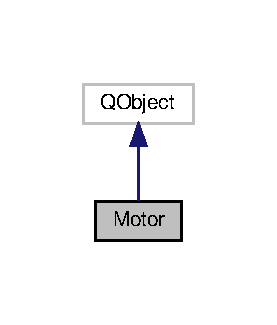
\includegraphics[width=133pt]{classMotor__inherit__graph}
\end{center}
\end{figure}


Collaboration diagram for Motor\+:
\nopagebreak
\begin{figure}[H]
\begin{center}
\leavevmode
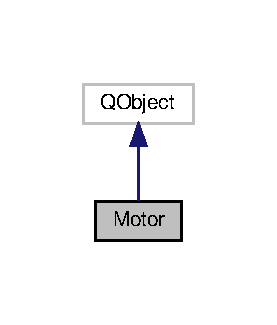
\includegraphics[width=133pt]{classMotor__coll__graph}
\end{center}
\end{figure}
\subsection*{Public Slots}
\begin{DoxyCompactItemize}
\item 
\mbox{\Hypertarget{classMotor_a6f235ed0f9e1ba51cc6cd1dcd823d850}\label{classMotor_a6f235ed0f9e1ba51cc6cd1dcd823d850}} 
void \hyperlink{classMotor_a6f235ed0f9e1ba51cc6cd1dcd823d850}{open} (Q\+String port)
\begin{DoxyCompactList}\small\item\em open establishes a connection over a serial port \end{DoxyCompactList}\item 
\mbox{\Hypertarget{classMotor_a6302ab51842ec23bd8b36d56e5ae9416}\label{classMotor_a6302ab51842ec23bd8b36d56e5ae9416}} 
void \hyperlink{classMotor_a6302ab51842ec23bd8b36d56e5ae9416}{close} ()
\begin{DoxyCompactList}\small\item\em close closes the serialport connection \end{DoxyCompactList}\item 
\mbox{\Hypertarget{classMotor_adc21685543cb0f520fec7291b4a642f0}\label{classMotor_adc21685543cb0f520fec7291b4a642f0}} 
void \hyperlink{classMotor_adc21685543cb0f520fec7291b4a642f0}{read} ()
\begin{DoxyCompactList}\small\item\em read reads from the serial port \end{DoxyCompactList}\item 
void \hyperlink{classMotor_a8305ead4b01433cb8a01eb5440a8b570}{write} (const Q\+Byte\+Array \&data)
\begin{DoxyCompactList}\small\item\em write writes to the serialport \end{DoxyCompactList}\item 
void \hyperlink{classMotor_a4c95080f6faf87f02844093e948d485a}{handle\+Error} (Q\+Serial\+Port\+::\+Serial\+Port\+Error error)
\begin{DoxyCompactList}\small\item\em handle\+Error prints an error message of the serialport connection and closes the connection \end{DoxyCompactList}\item 
void \hyperlink{classMotor_a3d9df9be923b64306fa28dff13ceaa2e}{show\+Status\+Message} (const Q\+String \&message)
\begin{DoxyCompactList}\small\item\em show\+Status\+Message fills the label in the G\+UI with text \end{DoxyCompactList}\item 
bool \hyperlink{classMotor_a6522462ca0730300ca3335090425786b}{isopen} ()
\begin{DoxyCompactList}\small\item\em isopen returns the state of the serial connection \end{DoxyCompactList}\item 
\mbox{\Hypertarget{classMotor_a1b3e37fc95517b98914ce3740232b098}\label{classMotor_a1b3e37fc95517b98914ce3740232b098}} 
void \hyperlink{classMotor_a1b3e37fc95517b98914ce3740232b098}{command\+\_\+park} ()
\begin{DoxyCompactList}\small\item\em command\+\_\+park moves the motor to the mechanical stop \end{DoxyCompactList}\item 
\mbox{\Hypertarget{classMotor_a75c8443fde45f5dc88e7bfe12db75a88}\label{classMotor_a75c8443fde45f5dc88e7bfe12db75a88}} 
void \hyperlink{classMotor_a75c8443fde45f5dc88e7bfe12db75a88}{command\+\_\+home} ()
\begin{DoxyCompactList}\small\item\em command\+\_\+home sends commands to position at the mechanical stop and afterwards go to the offset starting position, but in an inaccurate way \end{DoxyCompactList}\item 
\mbox{\Hypertarget{classMotor_abae5d9c4f4e3e9b67a98ca2486edacb9}\label{classMotor_abae5d9c4f4e3e9b67a98ca2486edacb9}} 
void \hyperlink{classMotor_abae5d9c4f4e3e9b67a98ca2486edacb9}{command\+\_\+info} ()
\begin{DoxyCompactList}\small\item\em command\+\_\+info sends the command to request the P\+C\+B\+Motor information \end{DoxyCompactList}\item 
\mbox{\Hypertarget{classMotor_aca8c344a7251cc4067f4d1cba69f7970}\label{classMotor_aca8c344a7251cc4067f4d1cba69f7970}} 
void \hyperlink{classMotor_aca8c344a7251cc4067f4d1cba69f7970}{command\+\_\+help} ()
\begin{DoxyCompactList}\small\item\em command\+\_\+help sends the command to print the P\+C\+B\+Motor help \end{DoxyCompactList}\item 
\mbox{\Hypertarget{classMotor_ade0bd3f46caadb9fef19f03629fc4e71}\label{classMotor_ade0bd3f46caadb9fef19f03629fc4e71}} 
void \hyperlink{classMotor_ade0bd3f46caadb9fef19f03629fc4e71}{command\+\_\+frequency\+\_\+sweep} ()
\begin{DoxyCompactList}\small\item\em command\+\_\+frequency\+\_\+sweep sends the P\+C\+B\+Motor command for a frequency sweep \end{DoxyCompactList}\item 
void \hyperlink{classMotor_ae052b079f5bd433c3561eb8b6d772b80}{command\+\_\+singlestep} (Q\+String dirstring)
\begin{DoxyCompactList}\small\item\em command\+\_\+singlestep moves the motor a single step in a direction specified by dirstring \end{DoxyCompactList}\item 
void \hyperlink{classMotor_aafbe8e02e29d2a81287747ae09b3d9fa}{command\+\_\+step} (uint16\+\_\+t numsteps, Q\+String dirstring)
\begin{DoxyCompactList}\small\item\em command\+\_\+step moves the motor numstep steps in a direction specified by dirstring \end{DoxyCompactList}\item 
void \hyperlink{classMotor_abfbe0b96cfb97107128084ec065e31c2}{command\+\_\+microstep} (uint16\+\_\+t nummsteps, Q\+String dirstring)
\begin{DoxyCompactList}\small\item\em command\+\_\+microstep aplies nummsteps micropulses to the motor \end{DoxyCompactList}\item 
void \hyperlink{classMotor_a9ca6508221ea2c42a5220848ab37df30}{stop} (bool stop)
\begin{DoxyCompactList}\small\item\em stop Tries to stop movenents if possible \end{DoxyCompactList}\item 
void \hyperlink{classMotor_a3d179f71c181cbeb3cdb44af166e532d}{command\+\_\+moveboth} (double ang1, double ang2)
\begin{DoxyCompactList}\small\item\em command\+\_\+moveboth moves both motors connected to the controller \end{DoxyCompactList}\end{DoxyCompactItemize}
\subsection*{Signals}
\begin{DoxyCompactItemize}
\item 
void \hyperlink{classMotor_ad12a639c95a4a33f59118dc8145dc1d4}{motorstatusmessage} (const Q\+String \&message)
\begin{DoxyCompactList}\small\item\em motorstatusmessage emitted when the status of the serial connection changes, with a string indicating the actual state. \end{DoxyCompactList}\item 
\mbox{\Hypertarget{classMotor_afcf83aa74380932f2408c150b806b5fb}\label{classMotor_afcf83aa74380932f2408c150b806b5fb}} 
void \hyperlink{classMotor_afcf83aa74380932f2408c150b806b5fb}{Connection\+Closed} ()
\begin{DoxyCompactList}\small\item\em emitted when serial connection is closed \end{DoxyCompactList}\end{DoxyCompactItemize}
\subsection*{Public Member Functions}
\begin{DoxyCompactItemize}
\item 
\mbox{\Hypertarget{classMotor_af6fb1d675035fd353cd2cb97dbdbecc9}\label{classMotor_af6fb1d675035fd353cd2cb97dbdbecc9}} 
\hyperlink{classMotor_af6fb1d675035fd353cd2cb97dbdbecc9}{Motor} ()
\begin{DoxyCompactList}\small\item\em \hyperlink{classMotor}{Motor} the contructor initializes variables and establishes the serial connection. \end{DoxyCompactList}\item 
bool \hyperlink{classMotor_a3e5e0ed8b8095588a09283200aaeb142}{sensordata} ()
\begin{DoxyCompactList}\small\item\em sensordata returns the current P\+C\+B\+Motor optical encoder wheel sendor state \end{DoxyCompactList}\end{DoxyCompactItemize}
\subsection*{Public Attributes}
\begin{DoxyCompactItemize}
\item 
\mbox{\Hypertarget{classMotor_ac64f7613ade081a22859151662b8e866}\label{classMotor_ac64f7613ade081a22859151662b8e866}} 
Q\+String \hyperlink{classMotor_ac64f7613ade081a22859151662b8e866}{publicmotorstatusmessage}
\begin{DoxyCompactList}\small\item\em A string containing the current state of the serial connection. \end{DoxyCompactList}\item 
\mbox{\Hypertarget{classMotor_a830ca5e3e68b7bc0ffb30650d72b8efb}\label{classMotor_a830ca5e3e68b7bc0ffb30650d72b8efb}} 
Q\+Serial\+Port $\ast$ \hyperlink{classMotor_a830ca5e3e68b7bc0ffb30650d72b8efb}{serial}
\begin{DoxyCompactList}\small\item\em Qt serial connection interface. \end{DoxyCompactList}\end{DoxyCompactItemize}
\subsection*{Private Member Functions}
\begin{DoxyCompactItemize}
\item 
\mbox{\Hypertarget{classMotor_a58e08c8118b2e3272c35086ac6289428}\label{classMotor_a58e08c8118b2e3272c35086ac6289428}} 
void \hyperlink{classMotor_a58e08c8118b2e3272c35086ac6289428}{moveboth} ()
\begin{DoxyCompactList}\small\item\em command\+\_\+moveboth moves both motors connected to the controller \end{DoxyCompactList}\end{DoxyCompactItemize}
\subsection*{Private Attributes}
\begin{DoxyCompactItemize}
\item 
Q\+Timer \hyperlink{classMotor_adbb59f89d592f1569ba8ad05c5c58a73}{hometimer}
\begin{DoxyCompactList}\small\item\em Used to iterate through the steps of \textquotesingle{}go to the starting position\textquotesingle{} -\/ but in an inaccurate way. \end{DoxyCompactList}\item 
\mbox{\Hypertarget{classMotor_a97bf769ce21887450f412554520f4f20}\label{classMotor_a97bf769ce21887450f412554520f4f20}} 
Q\+Timer \hyperlink{classMotor_a97bf769ce21887450f412554520f4f20}{bothtimer}
\begin{DoxyCompactList}\small\item\em Used to iterate through the steps of moving two motors of one controller. \end{DoxyCompactList}\item 
\mbox{\Hypertarget{classMotor_a64cf23f01da50ffdfd3c5ba26ad44f1f}\label{classMotor_a64cf23f01da50ffdfd3c5ba26ad44f1f}} 
int {\bfseries movebothstep}
\item 
\mbox{\Hypertarget{classMotor_a65cf2259e3d3e61ea7e268b99f8089a0}\label{classMotor_a65cf2259e3d3e61ea7e268b99f8089a0}} 
bool {\bfseries serialconnectionok}
\item 
\mbox{\Hypertarget{classMotor_a09aaad8e6e0ea959ac4712677443d8f0}\label{classMotor_a09aaad8e6e0ea959ac4712677443d8f0}} 
uint16\+\_\+t {\bfseries motor1steps}
\item 
\mbox{\Hypertarget{classMotor_af12031af563931e69915308aa0cce190}\label{classMotor_af12031af563931e69915308aa0cce190}} 
uint16\+\_\+t {\bfseries motor2steps}
\end{DoxyCompactItemize}


\subsection{Detailed Description}
The \hyperlink{classMotor}{Motor} class operates the P\+C\+B-\/motor. 

\begin{DoxyRefDesc}{Bug}
\item[\hyperlink{bug__bug000004}{Bug}]There are no known bugs.\end{DoxyRefDesc}


The P\+C\+B\+Motor is controllable by sending A\+S\+C\+II commands over a serial connection. This class establishes such a connection and controls the movements of the motor. 

\subsection{Member Function Documentation}
\mbox{\Hypertarget{classMotor_abfbe0b96cfb97107128084ec065e31c2}\label{classMotor_abfbe0b96cfb97107128084ec065e31c2}} 
\index{Motor@{Motor}!command\+\_\+microstep@{command\+\_\+microstep}}
\index{command\+\_\+microstep@{command\+\_\+microstep}!Motor@{Motor}}
\subsubsection{\texorpdfstring{command\+\_\+microstep}{command\_microstep}}
{\footnotesize\ttfamily void Motor\+::command\+\_\+microstep (\begin{DoxyParamCaption}\item[{uint16\+\_\+t}]{nummsteps,  }\item[{Q\+String}]{dirstring }\end{DoxyParamCaption})\hspace{0.3cm}{\ttfamily [slot]}}



command\+\_\+microstep aplies nummsteps micropulses to the motor 


\begin{DoxyParams}{Parameters}
{\em nummsteps} & number of micropulses to apply \\
\hline
{\em dirstring} & string containing the desired direction\\
\hline
\end{DoxyParams}
dirstring may either be \char`\"{}bw\char`\"{} of \char`\"{}fw\char`\"{} for backward/forward movement. \mbox{\Hypertarget{classMotor_a3d179f71c181cbeb3cdb44af166e532d}\label{classMotor_a3d179f71c181cbeb3cdb44af166e532d}} 
\index{Motor@{Motor}!command\+\_\+moveboth@{command\+\_\+moveboth}}
\index{command\+\_\+moveboth@{command\+\_\+moveboth}!Motor@{Motor}}
\subsubsection{\texorpdfstring{command\+\_\+moveboth}{command\_moveboth}}
{\footnotesize\ttfamily void Motor\+::command\+\_\+moveboth (\begin{DoxyParamCaption}\item[{double}]{ang1,  }\item[{double}]{ang2 }\end{DoxyParamCaption})\hspace{0.3cm}{\ttfamily [slot]}}



command\+\_\+moveboth moves both motors connected to the controller 


\begin{DoxyParams}{Parameters}
{\em ang1} & angle motor 1 is to be moved to \\
\hline
{\em ang2angle} & motor 2 is to be moved to \\
\hline
\end{DoxyParams}
\mbox{\Hypertarget{classMotor_ae052b079f5bd433c3561eb8b6d772b80}\label{classMotor_ae052b079f5bd433c3561eb8b6d772b80}} 
\index{Motor@{Motor}!command\+\_\+singlestep@{command\+\_\+singlestep}}
\index{command\+\_\+singlestep@{command\+\_\+singlestep}!Motor@{Motor}}
\subsubsection{\texorpdfstring{command\+\_\+singlestep}{command\_singlestep}}
{\footnotesize\ttfamily void Motor\+::command\+\_\+singlestep (\begin{DoxyParamCaption}\item[{Q\+String}]{dirstring }\end{DoxyParamCaption})\hspace{0.3cm}{\ttfamily [slot]}}



command\+\_\+singlestep moves the motor a single step in a direction specified by dirstring 


\begin{DoxyParams}{Parameters}
{\em dirstring} & a string containing the desired movenent direction\\
\hline
\end{DoxyParams}
Dirstring may either be \char`\"{}bw\char`\"{} of \char`\"{}fw\char`\"{} for backward/forward movement. \mbox{\Hypertarget{classMotor_aafbe8e02e29d2a81287747ae09b3d9fa}\label{classMotor_aafbe8e02e29d2a81287747ae09b3d9fa}} 
\index{Motor@{Motor}!command\+\_\+step@{command\+\_\+step}}
\index{command\+\_\+step@{command\+\_\+step}!Motor@{Motor}}
\subsubsection{\texorpdfstring{command\+\_\+step}{command\_step}}
{\footnotesize\ttfamily void Motor\+::command\+\_\+step (\begin{DoxyParamCaption}\item[{uint16\+\_\+t}]{numsteps,  }\item[{Q\+String}]{dirstring }\end{DoxyParamCaption})\hspace{0.3cm}{\ttfamily [slot]}}



command\+\_\+step moves the motor numstep steps in a direction specified by dirstring 


\begin{DoxyParams}{Parameters}
{\em numsteps} & number of steps to go \\
\hline
{\em dirstring} & direction to go\\
\hline
\end{DoxyParams}
Dirstring may either be \char`\"{}bw\char`\"{} of \char`\"{}fw\char`\"{} for backward/forward movement. \mbox{\Hypertarget{classMotor_a4c95080f6faf87f02844093e948d485a}\label{classMotor_a4c95080f6faf87f02844093e948d485a}} 
\index{Motor@{Motor}!handle\+Error@{handle\+Error}}
\index{handle\+Error@{handle\+Error}!Motor@{Motor}}
\subsubsection{\texorpdfstring{handle\+Error}{handleError}}
{\footnotesize\ttfamily void Motor\+::handle\+Error (\begin{DoxyParamCaption}\item[{Q\+Serial\+Port\+::\+Serial\+Port\+Error}]{error }\end{DoxyParamCaption})\hspace{0.3cm}{\ttfamily [slot]}}



handle\+Error prints an error message of the serialport connection and closes the connection 


\begin{DoxyParams}{Parameters}
{\em error} & \\
\hline
\end{DoxyParams}
\mbox{\Hypertarget{classMotor_a6522462ca0730300ca3335090425786b}\label{classMotor_a6522462ca0730300ca3335090425786b}} 
\index{Motor@{Motor}!isopen@{isopen}}
\index{isopen@{isopen}!Motor@{Motor}}
\subsubsection{\texorpdfstring{isopen}{isopen}}
{\footnotesize\ttfamily bool Motor\+::isopen (\begin{DoxyParamCaption}{ }\end{DoxyParamCaption})\hspace{0.3cm}{\ttfamily [slot]}}



isopen returns the state of the serial connection 

\begin{DoxyReturn}{Returns}
true if serial connection was established successfully, false otherwise 
\end{DoxyReturn}
\mbox{\Hypertarget{classMotor_ad12a639c95a4a33f59118dc8145dc1d4}\label{classMotor_ad12a639c95a4a33f59118dc8145dc1d4}} 
\index{Motor@{Motor}!motorstatusmessage@{motorstatusmessage}}
\index{motorstatusmessage@{motorstatusmessage}!Motor@{Motor}}
\subsubsection{\texorpdfstring{motorstatusmessage}{motorstatusmessage}}
{\footnotesize\ttfamily void Motor\+::motorstatusmessage (\begin{DoxyParamCaption}\item[{const Q\+String \&}]{message }\end{DoxyParamCaption})\hspace{0.3cm}{\ttfamily [signal]}}



motorstatusmessage emitted when the status of the serial connection changes, with a string indicating the actual state. 


\begin{DoxyParams}{Parameters}
{\em message} & the message \\
\hline
\end{DoxyParams}
\mbox{\Hypertarget{classMotor_a3e5e0ed8b8095588a09283200aaeb142}\label{classMotor_a3e5e0ed8b8095588a09283200aaeb142}} 
\index{Motor@{Motor}!sensordata@{sensordata}}
\index{sensordata@{sensordata}!Motor@{Motor}}
\subsubsection{\texorpdfstring{sensordata()}{sensordata()}}
{\footnotesize\ttfamily bool Motor\+::sensordata (\begin{DoxyParamCaption}{ }\end{DoxyParamCaption})}



sensordata returns the current P\+C\+B\+Motor optical encoder wheel sendor state 

\begin{DoxyReturn}{Returns}
the current P\+C\+B\+Motor optical encoder wheel sendor state 
\end{DoxyReturn}
\mbox{\Hypertarget{classMotor_a3d9df9be923b64306fa28dff13ceaa2e}\label{classMotor_a3d9df9be923b64306fa28dff13ceaa2e}} 
\index{Motor@{Motor}!show\+Status\+Message@{show\+Status\+Message}}
\index{show\+Status\+Message@{show\+Status\+Message}!Motor@{Motor}}
\subsubsection{\texorpdfstring{show\+Status\+Message}{showStatusMessage}}
{\footnotesize\ttfamily void Motor\+::show\+Status\+Message (\begin{DoxyParamCaption}\item[{const Q\+String \&}]{message }\end{DoxyParamCaption})\hspace{0.3cm}{\ttfamily [slot]}}



show\+Status\+Message fills the label in the G\+UI with text 


\begin{DoxyParams}{Parameters}
{\em message} & the text to be shown in the label \\
\hline
\end{DoxyParams}
\mbox{\Hypertarget{classMotor_a9ca6508221ea2c42a5220848ab37df30}\label{classMotor_a9ca6508221ea2c42a5220848ab37df30}} 
\index{Motor@{Motor}!stop@{stop}}
\index{stop@{stop}!Motor@{Motor}}
\subsubsection{\texorpdfstring{stop}{stop}}
{\footnotesize\ttfamily void Motor\+::stop (\begin{DoxyParamCaption}\item[{bool}]{stop }\end{DoxyParamCaption})\hspace{0.3cm}{\ttfamily [slot]}}



stop Tries to stop movenents if possible 


\begin{DoxyParams}{Parameters}
{\em stop} & Input\+: True if movents shall be stopped if possible \\
\hline
\end{DoxyParams}
\mbox{\Hypertarget{classMotor_a8305ead4b01433cb8a01eb5440a8b570}\label{classMotor_a8305ead4b01433cb8a01eb5440a8b570}} 
\index{Motor@{Motor}!write@{write}}
\index{write@{write}!Motor@{Motor}}
\subsubsection{\texorpdfstring{write}{write}}
{\footnotesize\ttfamily void Motor\+::write (\begin{DoxyParamCaption}\item[{const Q\+Byte\+Array \&}]{data }\end{DoxyParamCaption})\hspace{0.3cm}{\ttfamily [slot]}}



write writes to the serialport 


\begin{DoxyParams}{Parameters}
{\em data} & data to be written to the serial port \\
\hline
\end{DoxyParams}


\subsection{Member Data Documentation}
\mbox{\Hypertarget{classMotor_adbb59f89d592f1569ba8ad05c5c58a73}\label{classMotor_adbb59f89d592f1569ba8ad05c5c58a73}} 
\index{Motor@{Motor}!hometimer@{hometimer}}
\index{hometimer@{hometimer}!Motor@{Motor}}
\subsubsection{\texorpdfstring{hometimer}{hometimer}}
{\footnotesize\ttfamily Q\+Timer Motor\+::hometimer\hspace{0.3cm}{\ttfamily [private]}}



Used to iterate through the steps of \textquotesingle{}go to the starting position\textquotesingle{} -\/ but in an inaccurate way. 

\begin{DoxySeeAlso}{See also}
\hyperlink{classMotor_a75c8443fde45f5dc88e7bfe12db75a88}{command\+\_\+home()} 
\end{DoxySeeAlso}


The documentation for this class was generated from the following files\+:\begin{DoxyCompactItemize}
\item 
\hyperlink{motor_8h}{motor.\+h}\item 
motor.\+cpp\end{DoxyCompactItemize}

\hypertarget{classUDPlistener}{}\section{U\+D\+Plistener Class Reference}
\label{classUDPlistener}\index{U\+D\+Plistener@{U\+D\+Plistener}}


The \hyperlink{classUDPlistener}{U\+D\+Plistener} class is used to control dinspect with U\+DP packages.  




{\ttfamily \#include $<$udplistener.\+h$>$}



Inheritance diagram for U\+D\+Plistener\+:
\nopagebreak
\begin{figure}[H]
\begin{center}
\leavevmode
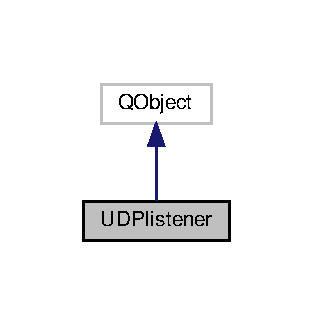
\includegraphics[width=150pt]{classUDPlistener__inherit__graph}
\end{center}
\end{figure}


Collaboration diagram for U\+D\+Plistener\+:
\nopagebreak
\begin{figure}[H]
\begin{center}
\leavevmode
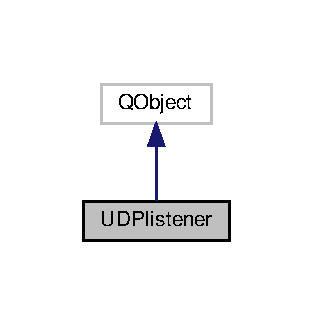
\includegraphics[width=150pt]{classUDPlistener__coll__graph}
\end{center}
\end{figure}
\subsection*{Public Slots}
\begin{DoxyCompactItemize}
\item 
void \hyperlink{classUDPlistener_a4b7a056403f9b80485c92b82c340109a}{bind} ()
\begin{DoxyCompactList}\small\item\em bind Binds to a new U\+DP port \end{DoxyCompactList}\end{DoxyCompactItemize}
\subsection*{Signals}
\begin{DoxyCompactItemize}
\item 
void \hyperlink{classUDPlistener_a03cb7a923fb064f41395f8db9409e511}{Move} (Q\+String controller, double H\+W\+Pang, double Q\+W\+Pang)
\begin{DoxyCompactList}\small\item\em Move moves the waveplates in a cage to certain angles. \end{DoxyCompactList}\item 
void \hyperlink{classUDPlistener_a3d16ae857b48ba56257008a008b4e6ee}{Move\+HV} (Q\+String controller)
\begin{DoxyCompactList}\small\item\em Move\+HV moves cage to H/V basis. \end{DoxyCompactList}\item 
void \hyperlink{classUDPlistener_a3e3521c57796737bb229eeadb2f2fdfe}{Move\+PM} (Q\+String controller)
\begin{DoxyCompactList}\small\item\em Move\+PM moves cage to P/M basis. \end{DoxyCompactList}\item 
void \hyperlink{classUDPlistener_aefb57eacf9148d294952db636eefa9ac}{Move\+LR} (Q\+String controller)
\begin{DoxyCompactList}\small\item\em Move\+LR moves cage to R/L basis. \end{DoxyCompactList}\end{DoxyCompactItemize}
\subsection*{Public Member Functions}
\begin{DoxyCompactItemize}
\item 
\hyperlink{classUDPlistener_a789cb6a7b7347a2df5cdc85a457bde4a}{U\+D\+Plistener} (Q\+Settings $\ast$\hyperlink{classUDPlistener_a14614017bcc3fc38e0caad8d4a9781a6}{settings}, Q\+Object $\ast$parent=0)
\begin{DoxyCompactList}\small\item\em \hyperlink{classUDPlistener}{U\+D\+Plistener} listen for commands on a U\+DP port and execute them. \end{DoxyCompactList}\end{DoxyCompactItemize}
\subsection*{Private Slots}
\begin{DoxyCompactItemize}
\item 
\mbox{\Hypertarget{classUDPlistener_ac971ee184440cfc88ff260db8ca3a2ca}\label{classUDPlistener_ac971ee184440cfc88ff260db8ca3a2ca}} 
void \hyperlink{classUDPlistener_ac971ee184440cfc88ff260db8ca3a2ca}{process\+Pending\+Datagrams} ()
\begin{DoxyCompactList}\small\item\em process\+Pending\+Datagrams reads data from the U\+DP socket \end{DoxyCompactList}\item 
void \hyperlink{classUDPlistener_a86e1147a1adf1a32ae49d43529cd53f1}{process\+Commands} (Q\+String msg)
\begin{DoxyCompactList}\small\item\em process\+Commands extracts commands out of received data and executes them \end{DoxyCompactList}\end{DoxyCompactItemize}
\subsection*{Private Attributes}
\begin{DoxyCompactItemize}
\item 
\mbox{\Hypertarget{classUDPlistener_a14614017bcc3fc38e0caad8d4a9781a6}\label{classUDPlistener_a14614017bcc3fc38e0caad8d4a9781a6}} 
Q\+Settings $\ast$ \hyperlink{classUDPlistener_a14614017bcc3fc38e0caad8d4a9781a6}{settings}
\begin{DoxyCompactList}\small\item\em configuration \end{DoxyCompactList}\item 
\mbox{\Hypertarget{classUDPlistener_a4e391608821969dc58f1cf509d0206fd}\label{classUDPlistener_a4e391608821969dc58f1cf509d0206fd}} 
Q\+Udp\+Socket \hyperlink{classUDPlistener_a4e391608821969dc58f1cf509d0206fd}{socket}
\begin{DoxyCompactList}\small\item\em the U\+DP socket \end{DoxyCompactList}\item 
\mbox{\Hypertarget{classUDPlistener_ab1fb04f4812b70f607727e27cedf26b1}\label{classUDPlistener_ab1fb04f4812b70f607727e27cedf26b1}} 
uint \hyperlink{classUDPlistener_ab1fb04f4812b70f607727e27cedf26b1}{port}
\begin{DoxyCompactList}\small\item\em port the listener listens to \end{DoxyCompactList}\item 
\mbox{\Hypertarget{classUDPlistener_ad032b16f2451215e0f4bd7b6998fc11d}\label{classUDPlistener_ad032b16f2451215e0f4bd7b6998fc11d}} 
bool \hyperlink{classUDPlistener_ad032b16f2451215e0f4bd7b6998fc11d}{alreadybound}
\begin{DoxyCompactList}\small\item\em true if the listener is already listening to a port \end{DoxyCompactList}\end{DoxyCompactItemize}


\subsection{Detailed Description}
The \hyperlink{classUDPlistener}{U\+D\+Plistener} class is used to control dinspect with U\+DP packages. 

\begin{DoxyRefDesc}{Bug}
\item[\hyperlink{bug__bug000005}{Bug}]There are no known bugs\end{DoxyRefDesc}


\subsection{Constructor \& Destructor Documentation}
\mbox{\Hypertarget{classUDPlistener_a789cb6a7b7347a2df5cdc85a457bde4a}\label{classUDPlistener_a789cb6a7b7347a2df5cdc85a457bde4a}} 
\index{U\+D\+Plistener@{U\+D\+Plistener}!U\+D\+Plistener@{U\+D\+Plistener}}
\index{U\+D\+Plistener@{U\+D\+Plistener}!U\+D\+Plistener@{U\+D\+Plistener}}
\subsubsection{\texorpdfstring{U\+D\+Plistener()}{UDPlistener()}}
{\footnotesize\ttfamily U\+D\+Plistener\+::\+U\+D\+Plistener (\begin{DoxyParamCaption}\item[{Q\+Settings $\ast$}]{settings,  }\item[{Q\+Object $\ast$}]{parent = {\ttfamily 0} }\end{DoxyParamCaption})\hspace{0.3cm}{\ttfamily [explicit]}}



\hyperlink{classUDPlistener}{U\+D\+Plistener} listen for commands on a U\+DP port and execute them. 


\begin{DoxyParams}{Parameters}
{\em settings} & a pointer to a qsettings instance, used to get the port to bind to and known commands\\
\hline
\end{DoxyParams}
\hyperlink{classUDPlistener}{U\+D\+Plistener} opens a U\+DP socket and binds to a port specified in qsettings. Incoming packages are analysed to check if they contain known commands. If they do, these commands are executed.

The commands can be changed in the dinspect settings dialog, but the standard ones are\+:
\begin{DoxyItemize}
\item Move(\+Q\+String, Q\+String)
\item \hyperlink{classUDPlistener_a03cb7a923fb064f41395f8db9409e511}{Move(\+Q\+String, double, double)} 
\end{DoxyItemize}

\subsection{Member Function Documentation}
\mbox{\Hypertarget{classUDPlistener_a4b7a056403f9b80485c92b82c340109a}\label{classUDPlistener_a4b7a056403f9b80485c92b82c340109a}} 
\index{U\+D\+Plistener@{U\+D\+Plistener}!bind@{bind}}
\index{bind@{bind}!U\+D\+Plistener@{U\+D\+Plistener}}
\subsubsection{\texorpdfstring{bind}{bind}}
{\footnotesize\ttfamily void U\+D\+Plistener\+::bind (\begin{DoxyParamCaption}{ }\end{DoxyParamCaption})\hspace{0.3cm}{\ttfamily [slot]}}



bind Binds to a new U\+DP port 

This function checks whether the U\+DP socket is already bound to a a specific port. If so, it closes this connection and binds to the new port. If not, it binds to the port right away. \mbox{\Hypertarget{classUDPlistener_a03cb7a923fb064f41395f8db9409e511}\label{classUDPlistener_a03cb7a923fb064f41395f8db9409e511}} 
\index{U\+D\+Plistener@{U\+D\+Plistener}!Move@{Move}}
\index{Move@{Move}!U\+D\+Plistener@{U\+D\+Plistener}}
\subsubsection{\texorpdfstring{Move}{Move}}
{\footnotesize\ttfamily void U\+D\+Plistener\+::\+Move (\begin{DoxyParamCaption}\item[{Q\+String}]{controller,  }\item[{double}]{H\+W\+Pang,  }\item[{double}]{Q\+W\+Pang }\end{DoxyParamCaption})\hspace{0.3cm}{\ttfamily [signal]}}



Move moves the waveplates in a cage to certain angles. 


\begin{DoxyParams}{Parameters}
{\em controller} & either colorcode of cage or \textquotesingle{}all\textquotesingle{} \\
\hline
{\em H\+W\+Pang} & angle of the H\+WP in degree \\
\hline
{\em Q\+W\+Pang} & angle of the Q\+WP in degree \\
\hline
\end{DoxyParams}
\mbox{\Hypertarget{classUDPlistener_a3d16ae857b48ba56257008a008b4e6ee}\label{classUDPlistener_a3d16ae857b48ba56257008a008b4e6ee}} 
\index{U\+D\+Plistener@{U\+D\+Plistener}!Move\+HV@{Move\+HV}}
\index{Move\+HV@{Move\+HV}!U\+D\+Plistener@{U\+D\+Plistener}}
\subsubsection{\texorpdfstring{Move\+HV}{MoveHV}}
{\footnotesize\ttfamily void U\+D\+Plistener\+::\+Move\+HV (\begin{DoxyParamCaption}\item[{Q\+String}]{controller }\end{DoxyParamCaption})\hspace{0.3cm}{\ttfamily [signal]}}



Move\+HV moves cage to H/V basis. 


\begin{DoxyParams}{Parameters}
{\em controller} & either colorcode of stage, or \textquotesingle{}all\textquotesingle{} \\
\hline
\end{DoxyParams}
\mbox{\Hypertarget{classUDPlistener_aefb57eacf9148d294952db636eefa9ac}\label{classUDPlistener_aefb57eacf9148d294952db636eefa9ac}} 
\index{U\+D\+Plistener@{U\+D\+Plistener}!Move\+LR@{Move\+LR}}
\index{Move\+LR@{Move\+LR}!U\+D\+Plistener@{U\+D\+Plistener}}
\subsubsection{\texorpdfstring{Move\+LR}{MoveLR}}
{\footnotesize\ttfamily void U\+D\+Plistener\+::\+Move\+LR (\begin{DoxyParamCaption}\item[{Q\+String}]{controller }\end{DoxyParamCaption})\hspace{0.3cm}{\ttfamily [signal]}}



Move\+LR moves cage to R/L basis. 


\begin{DoxyParams}{Parameters}
{\em controller} & either colorcode of stage, or \textquotesingle{}all\textquotesingle{} \\
\hline
\end{DoxyParams}
\mbox{\Hypertarget{classUDPlistener_a3e3521c57796737bb229eeadb2f2fdfe}\label{classUDPlistener_a3e3521c57796737bb229eeadb2f2fdfe}} 
\index{U\+D\+Plistener@{U\+D\+Plistener}!Move\+PM@{Move\+PM}}
\index{Move\+PM@{Move\+PM}!U\+D\+Plistener@{U\+D\+Plistener}}
\subsubsection{\texorpdfstring{Move\+PM}{MovePM}}
{\footnotesize\ttfamily void U\+D\+Plistener\+::\+Move\+PM (\begin{DoxyParamCaption}\item[{Q\+String}]{controller }\end{DoxyParamCaption})\hspace{0.3cm}{\ttfamily [signal]}}



Move\+PM moves cage to P/M basis. 


\begin{DoxyParams}{Parameters}
{\em controller} & either colorcode of stage, or \textquotesingle{}all\textquotesingle{} \\
\hline
\end{DoxyParams}
\mbox{\Hypertarget{classUDPlistener_a86e1147a1adf1a32ae49d43529cd53f1}\label{classUDPlistener_a86e1147a1adf1a32ae49d43529cd53f1}} 
\index{U\+D\+Plistener@{U\+D\+Plistener}!process\+Commands@{process\+Commands}}
\index{process\+Commands@{process\+Commands}!U\+D\+Plistener@{U\+D\+Plistener}}
\subsubsection{\texorpdfstring{process\+Commands}{processCommands}}
{\footnotesize\ttfamily void U\+D\+Plistener\+::process\+Commands (\begin{DoxyParamCaption}\item[{Q\+String}]{msg }\end{DoxyParamCaption})\hspace{0.3cm}{\ttfamily [private]}, {\ttfamily [slot]}}



process\+Commands extracts commands out of received data and executes them 


\begin{DoxyParams}{Parameters}
{\em msg} & input\+: the received message \\
\hline
\end{DoxyParams}


The documentation for this class was generated from the following files\+:\begin{DoxyCompactItemize}
\item 
\hyperlink{udplistener_8h}{udplistener.\+h}\item 
udplistener.\+cpp\end{DoxyCompactItemize}

\chapter{File Documentation}
\hypertarget{debug_8h}{}\section{debug.\+h File Reference}
\label{debug_8h}\index{debug.\+h@{debug.\+h}}


contains debug macros  


{\ttfamily \#include \char`\"{}stdio.\+h\char`\"{}}\newline
{\ttfamily \#include \char`\"{}defines.\+h\char`\"{}}\newline
Include dependency graph for debug.\+h\+:
\nopagebreak
\begin{figure}[H]
\begin{center}
\leavevmode
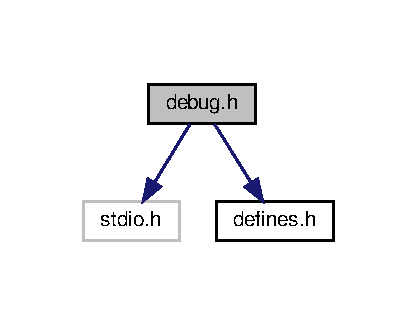
\includegraphics[width=200pt]{debug_8h__incl}
\end{center}
\end{figure}
This graph shows which files directly or indirectly include this file\+:
\nopagebreak
\begin{figure}[H]
\begin{center}
\leavevmode
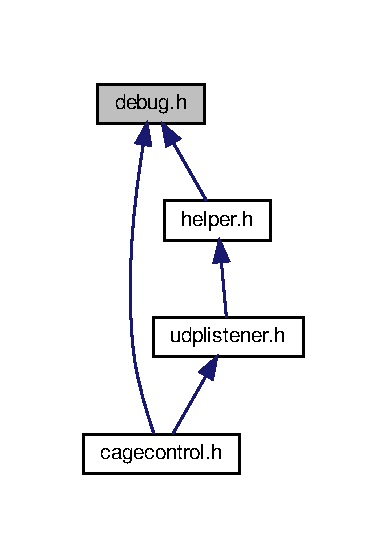
\includegraphics[width=224pt]{debug_8h__dep__incl}
\end{center}
\end{figure}


\subsection{Detailed Description}
contains debug macros 

\begin{DoxyRefDesc}{Bug}
\item[\hyperlink{bug__bug000001}{Bug}]Printing to console does not work on Windows. Workaround\+: Redirect stderr to stdout and redirect stdout to a file.\end{DoxyRefDesc}


This file defines macros to style and simplify output to console. 
\hypertarget{defines_8h}{}\section{defines.\+h File Reference}
\label{defines_8h}\index{defines.\+h@{defines.\+h}}


Various compile-\/time definitions.  


This graph shows which files directly or indirectly include this file\+:
\nopagebreak
\begin{figure}[H]
\begin{center}
\leavevmode
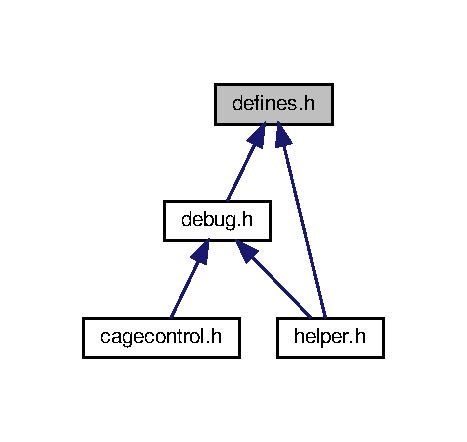
\includegraphics[width=238pt]{defines_8h__dep__incl}
\end{center}
\end{figure}
\subsection*{Macros}
\begin{DoxyCompactItemize}
\item 
\mbox{\Hypertarget{defines_8h_a78b073f863b42046c2f5c213502bf66c}\label{defines_8h_a78b073f863b42046c2f5c213502bf66c}} 
\#define {\bfseries D\+E\+B\+U\+G\+S\+P\+E\+C\+T\+R\+O\+M\+E\+T\+E\+R\+C\+O\+N\+F\+IG}~F\+A\+L\+SE
\item 
\#define \hyperlink{defines_8h_aea1d71af1a30c261dbd16745c82e94ba}{U\+N\+U\+S\+ED}(expr)~do \{ (void)(expr); \} while (0)
\item 
\#define \hyperlink{defines_8h_ad72dbcf6d0153db1b8d8a58001feed83}{D\+E\+B\+UG}~1
\item 
\#define \hyperlink{defines_8h_ac2aa26b507687122d58648153582d82e}{D\+E\+B\+U\+G\+E\+R\+R\+OR}~1
\item 
\#define \hyperlink{defines_8h_a4d33f6a22fa2272e18c3ffc0a1d30f59}{D\+E\+B\+U\+G\+W\+A\+R\+N\+I\+NG}~1
\item 
\#define \hyperlink{defines_8h_acc3775aea93cde2af0ced3225b4a0313}{D\+E\+B\+U\+G\+I\+N\+FO}~1
\item 
\#define \hyperlink{defines_8h_a6ebf6899d6c1c8b7b9d09be872c05aae}{E\+PS}~0.\+0000001
\item 
\#define \hyperlink{defines_8h_a598a3330b3c21701223ee0ca14316eca}{PI}~3.\+14159265358979323846
\item 
\#define \hyperlink{defines_8h_abbfb1b8e88373781c6238d647110f5d2}{D\+E\+G\+T\+O\+R\+AD}~\hyperlink{defines_8h_a598a3330b3c21701223ee0ca14316eca}{PI}/180
\item 
\#define \hyperlink{defines_8h_a9fcbc53371e9a60b983c6b338537aa40}{R\+A\+D\+T\+O\+D\+EG}~180/\hyperlink{defines_8h_a598a3330b3c21701223ee0ca14316eca}{PI}
\end{DoxyCompactItemize}


\subsection{Detailed Description}
Various compile-\/time definitions. 

\begin{DoxyRefDesc}{Bug}
\item[\hyperlink{bug__bug000002}{Bug}]There are no known bugs.\end{DoxyRefDesc}


Contains definitions of various kind -\/ mathematical, version constants, debug-\/variables, ... 

\subsection{Macro Definition Documentation}
\mbox{\Hypertarget{defines_8h_ad72dbcf6d0153db1b8d8a58001feed83}\label{defines_8h_ad72dbcf6d0153db1b8d8a58001feed83}} 
\index{defines.\+h@{defines.\+h}!D\+E\+B\+UG@{D\+E\+B\+UG}}
\index{D\+E\+B\+UG@{D\+E\+B\+UG}!defines.\+h@{defines.\+h}}
\subsubsection{\texorpdfstring{D\+E\+B\+UG}{DEBUG}}
{\footnotesize\ttfamily \#define D\+E\+B\+UG~1}

Enables the execution of various debug-\/paths used during development.~\newline
default\+: F\+A\+L\+SE. \mbox{\Hypertarget{defines_8h_ac2aa26b507687122d58648153582d82e}\label{defines_8h_ac2aa26b507687122d58648153582d82e}} 
\index{defines.\+h@{defines.\+h}!D\+E\+B\+U\+G\+E\+R\+R\+OR@{D\+E\+B\+U\+G\+E\+R\+R\+OR}}
\index{D\+E\+B\+U\+G\+E\+R\+R\+OR@{D\+E\+B\+U\+G\+E\+R\+R\+OR}!defines.\+h@{defines.\+h}}
\subsubsection{\texorpdfstring{D\+E\+B\+U\+G\+E\+R\+R\+OR}{DEBUGERROR}}
{\footnotesize\ttfamily \#define D\+E\+B\+U\+G\+E\+R\+R\+OR~1}

If set to T\+R\+UE, enables the execution of the D\+E\+B\+U\+G\+\_\+\+E\+R\+R\+O\+R() makro which is used to write error messages (critical) to stdout.~\newline
default\+: true \mbox{\Hypertarget{defines_8h_acc3775aea93cde2af0ced3225b4a0313}\label{defines_8h_acc3775aea93cde2af0ced3225b4a0313}} 
\index{defines.\+h@{defines.\+h}!D\+E\+B\+U\+G\+I\+N\+FO@{D\+E\+B\+U\+G\+I\+N\+FO}}
\index{D\+E\+B\+U\+G\+I\+N\+FO@{D\+E\+B\+U\+G\+I\+N\+FO}!defines.\+h@{defines.\+h}}
\subsubsection{\texorpdfstring{D\+E\+B\+U\+G\+I\+N\+FO}{DEBUGINFO}}
{\footnotesize\ttfamily \#define D\+E\+B\+U\+G\+I\+N\+FO~1}

If set to T\+R\+UE, enables the execution of the D\+E\+B\+U\+G\+\_\+\+I\+N\+F\+O() makro which is used to write usefull information to stdout.~\newline
default\+: true \mbox{\Hypertarget{defines_8h_a4d33f6a22fa2272e18c3ffc0a1d30f59}\label{defines_8h_a4d33f6a22fa2272e18c3ffc0a1d30f59}} 
\index{defines.\+h@{defines.\+h}!D\+E\+B\+U\+G\+W\+A\+R\+N\+I\+NG@{D\+E\+B\+U\+G\+W\+A\+R\+N\+I\+NG}}
\index{D\+E\+B\+U\+G\+W\+A\+R\+N\+I\+NG@{D\+E\+B\+U\+G\+W\+A\+R\+N\+I\+NG}!defines.\+h@{defines.\+h}}
\subsubsection{\texorpdfstring{D\+E\+B\+U\+G\+W\+A\+R\+N\+I\+NG}{DEBUGWARNING}}
{\footnotesize\ttfamily \#define D\+E\+B\+U\+G\+W\+A\+R\+N\+I\+NG~1}

If set to T\+R\+UE, enables the execution of the D\+E\+B\+U\+G\+\_\+\+W\+A\+R\+N\+I\+N\+G() makro which is used to write warnings about unexpected behaviour to stdout.~\newline
default\+: true \mbox{\Hypertarget{defines_8h_abbfb1b8e88373781c6238d647110f5d2}\label{defines_8h_abbfb1b8e88373781c6238d647110f5d2}} 
\index{defines.\+h@{defines.\+h}!D\+E\+G\+T\+O\+R\+AD@{D\+E\+G\+T\+O\+R\+AD}}
\index{D\+E\+G\+T\+O\+R\+AD@{D\+E\+G\+T\+O\+R\+AD}!defines.\+h@{defines.\+h}}
\subsubsection{\texorpdfstring{D\+E\+G\+T\+O\+R\+AD}{DEGTORAD}}
{\footnotesize\ttfamily \#define D\+E\+G\+T\+O\+R\+AD~\hyperlink{defines_8h_a598a3330b3c21701223ee0ca14316eca}{PI}/180}

Conversion factor from degree to radians. P\+I/180 \mbox{\Hypertarget{defines_8h_a6ebf6899d6c1c8b7b9d09be872c05aae}\label{defines_8h_a6ebf6899d6c1c8b7b9d09be872c05aae}} 
\index{defines.\+h@{defines.\+h}!E\+PS@{E\+PS}}
\index{E\+PS@{E\+PS}!defines.\+h@{defines.\+h}}
\subsubsection{\texorpdfstring{E\+PS}{EPS}}
{\footnotesize\ttfamily \#define E\+PS~0.\+0000001}

\textquotesingle{}epsilon\textquotesingle{} used to check floatingpoint variables in if-\/conditions.~\newline
default\+: 0.\+0000001 \mbox{\Hypertarget{defines_8h_a598a3330b3c21701223ee0ca14316eca}\label{defines_8h_a598a3330b3c21701223ee0ca14316eca}} 
\index{defines.\+h@{defines.\+h}!PI@{PI}}
\index{PI@{PI}!defines.\+h@{defines.\+h}}
\subsubsection{\texorpdfstring{PI}{PI}}
{\footnotesize\ttfamily \#define PI~3.\+14159265358979323846}

Pi.~\newline
default\+: 3.\+14159265358979323846 \mbox{\Hypertarget{defines_8h_a9fcbc53371e9a60b983c6b338537aa40}\label{defines_8h_a9fcbc53371e9a60b983c6b338537aa40}} 
\index{defines.\+h@{defines.\+h}!R\+A\+D\+T\+O\+D\+EG@{R\+A\+D\+T\+O\+D\+EG}}
\index{R\+A\+D\+T\+O\+D\+EG@{R\+A\+D\+T\+O\+D\+EG}!defines.\+h@{defines.\+h}}
\subsubsection{\texorpdfstring{R\+A\+D\+T\+O\+D\+EG}{RADTODEG}}
{\footnotesize\ttfamily \#define R\+A\+D\+T\+O\+D\+EG~180/\hyperlink{defines_8h_a598a3330b3c21701223ee0ca14316eca}{PI}}

Conversion factor from radians to degree. 180/\+PI \mbox{\Hypertarget{defines_8h_aea1d71af1a30c261dbd16745c82e94ba}\label{defines_8h_aea1d71af1a30c261dbd16745c82e94ba}} 
\index{defines.\+h@{defines.\+h}!U\+N\+U\+S\+ED@{U\+N\+U\+S\+ED}}
\index{U\+N\+U\+S\+ED@{U\+N\+U\+S\+ED}!defines.\+h@{defines.\+h}}
\subsubsection{\texorpdfstring{U\+N\+U\+S\+ED}{UNUSED}}
{\footnotesize\ttfamily \#define U\+N\+U\+S\+ED(\begin{DoxyParamCaption}\item[{}]{expr }\end{DoxyParamCaption})~do \{ (void)(expr); \} while (0)}

Use \hyperlink{defines_8h_aea1d71af1a30c261dbd16745c82e94ba}{U\+N\+U\+S\+E\+D(var)} in function f(...,type var,...) to silence compiler warnings about unused parameter var. 
\hypertarget{helper_8h}{}\section{helper.\+h File Reference}
\label{helper_8h}\index{helper.\+h@{helper.\+h}}
{\ttfamily \#include \char`\"{}debug.\+h\char`\"{}}\newline
{\ttfamily \#include \char`\"{}defines.\+h\char`\"{}}\newline
{\ttfamily \#include $<$Q\+Message\+Box$>$}\newline
Include dependency graph for helper.\+h\+:\nopagebreak
\begin{figure}[H]
\begin{center}
\leavevmode
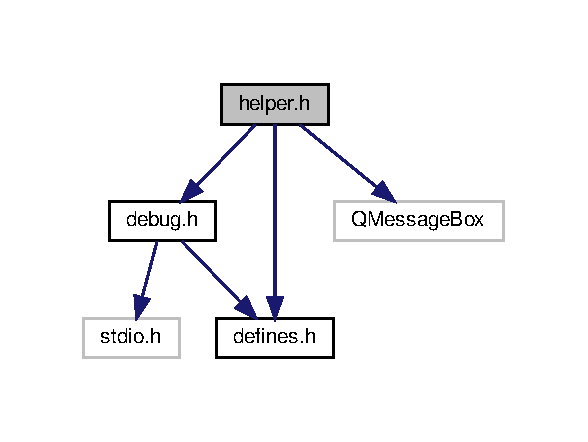
\includegraphics[width=282pt]{helper_8h__incl}
\end{center}
\end{figure}
This graph shows which files directly or indirectly include this file\+:\nopagebreak
\begin{figure}[H]
\begin{center}
\leavevmode
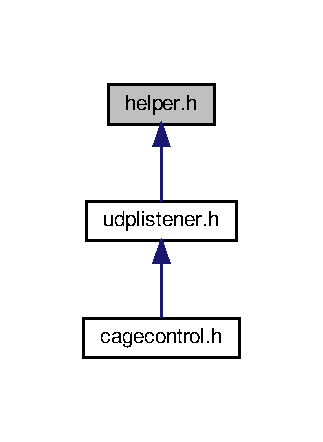
\includegraphics[width=155pt]{helper_8h__dep__incl}
\end{center}
\end{figure}
\subsection*{Namespaces}
\begin{DoxyCompactItemize}
\item 
 \hyperlink{namespacehelper}{helper}
\begin{DoxyCompactList}\small\item\em contains small functions to display messages \end{DoxyCompactList}\end{DoxyCompactItemize}
\subsection*{Functions}
\begin{DoxyCompactItemize}
\item 
void \hyperlink{namespacehelper_ab2cc8239d9bf2ae383474c0343205346}{helper\+::message} (Q\+String msg)
\begin{DoxyCompactList}\small\item\em message displays a message box \end{DoxyCompactList}\item 
void \hyperlink{namespacehelper_a00e308809a0f9d76f3a0ba2ad5f3587c}{helper\+::error} (Q\+String msg)
\begin{DoxyCompactList}\small\item\em error displays an error-\/messagebox and writes a debug\+\_\+error message to stdout \end{DoxyCompactList}\item 
void \hyperlink{namespacehelper_ac717f710dcb45bf31fba9071ea4fb45f}{helper\+::warning} (Q\+String msg)
\begin{DoxyCompactList}\small\item\em warning displays warning-\/messagebox and writes a debug\+\_\+warning message to stdout \end{DoxyCompactList}\item 
void \hyperlink{namespacehelper_a88e86d2fd14fc8354c1529beaa157f25}{helper\+::info} (Q\+String msg)
\begin{DoxyCompactList}\small\item\em info displays an info-\/messagebox and writes a debug\+\_\+info message to stdout \end{DoxyCompactList}\end{DoxyCompactItemize}

\hypertarget{motor_8h}{}\section{motor.\+h File Reference}
\label{motor_8h}\index{motor.\+h@{motor.\+h}}
{\ttfamily \#include $<$Q\+Dialog$>$}\newline
{\ttfamily \#include $<$Qt\+Core/\+Qt\+Global$>$}\newline
{\ttfamily \#include $<$Qt\+Serial\+Port/\+Q\+Serial\+Port$>$}\newline
{\ttfamily \#include $<$Q\+Object$>$}\newline
{\ttfamily \#include $<$Q\+Timer$>$}\newline
{\ttfamily \#include \char`\"{}defines.\+h\char`\"{}}\newline
Include dependency graph for motor.\+h\+:\nopagebreak
\begin{figure}[H]
\begin{center}
\leavevmode
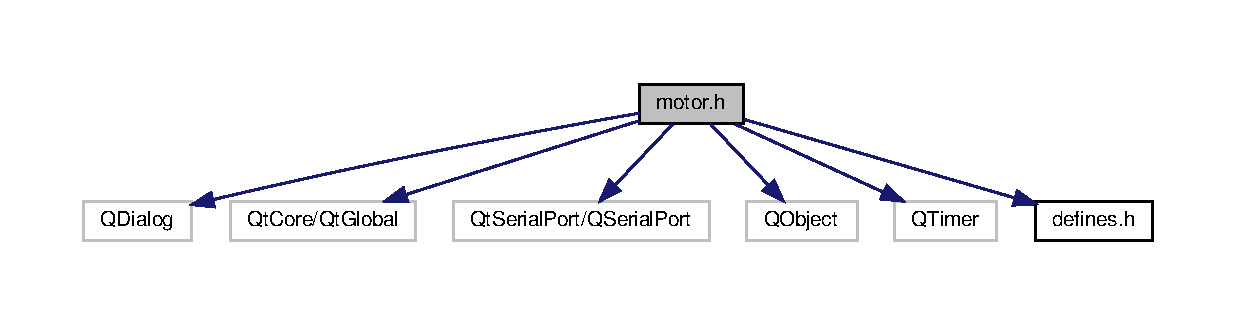
\includegraphics[width=350pt]{motor_8h__incl}
\end{center}
\end{figure}
This graph shows which files directly or indirectly include this file\+:
\nopagebreak
\begin{figure}[H]
\begin{center}
\leavevmode
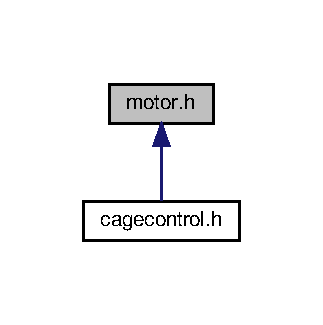
\includegraphics[width=155pt]{motor_8h__dep__incl}
\end{center}
\end{figure}
\subsection*{Classes}
\begin{DoxyCompactItemize}
\item 
class \hyperlink{classMotor}{Motor}
\begin{DoxyCompactList}\small\item\em The \hyperlink{classMotor}{Motor} class operates the P\+C\+B-\/motor. \end{DoxyCompactList}\end{DoxyCompactItemize}

\hypertarget{udplistener_8h}{}\section{udplistener.\+h File Reference}
\label{udplistener_8h}\index{udplistener.\+h@{udplistener.\+h}}
{\ttfamily \#include $<$Q\+Object$>$}\newline
{\ttfamily \#include $<$Q\+Host\+Address$>$}\newline
{\ttfamily \#include $<$Q\+Settings$>$}\newline
{\ttfamily \#include $<$Q\+Udp\+Socket$>$}\newline
{\ttfamily \#include \char`\"{}helper.\+h\char`\"{}}\newline
Include dependency graph for udplistener.\+h\+:\nopagebreak
\begin{figure}[H]
\begin{center}
\leavevmode
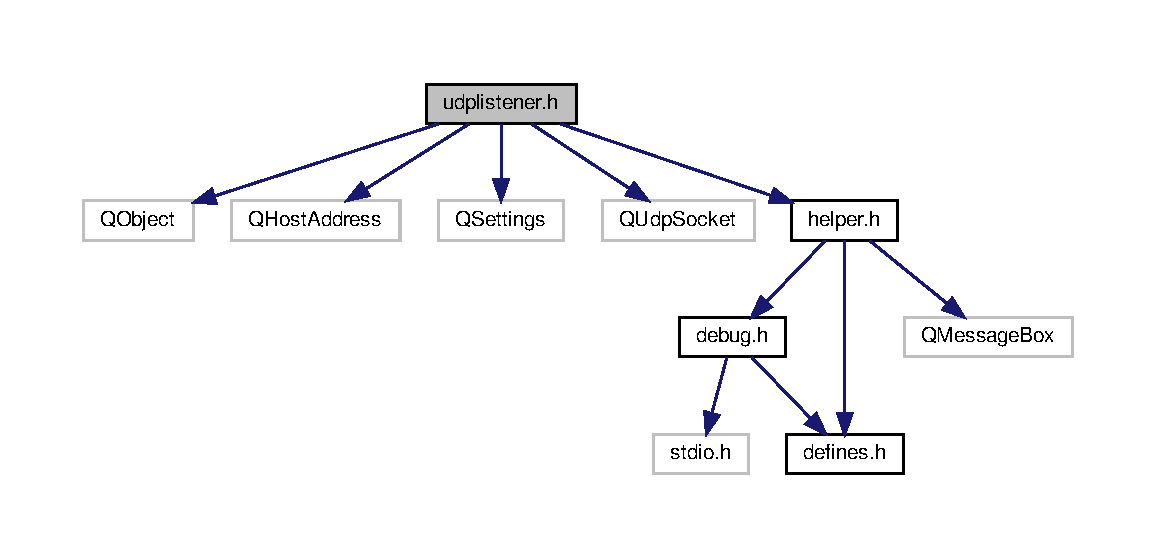
\includegraphics[width=350pt]{udplistener_8h__incl}
\end{center}
\end{figure}
This graph shows which files directly or indirectly include this file\+:\nopagebreak
\begin{figure}[H]
\begin{center}
\leavevmode
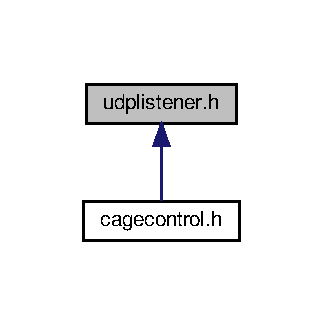
\includegraphics[width=155pt]{udplistener_8h__dep__incl}
\end{center}
\end{figure}
\subsection*{Classes}
\begin{DoxyCompactItemize}
\item 
class \hyperlink{classUDPlistener}{U\+D\+Plistener}
\begin{DoxyCompactList}\small\item\em The \hyperlink{classUDPlistener}{U\+D\+Plistener} class is used to control dinspect with U\+DP packages. \end{DoxyCompactList}\end{DoxyCompactItemize}

\hypertarget{version_8h}{}\section{version.\+h File Reference}
\label{version_8h}\index{version.\+h@{version.\+h}}


This file contains information about the code version.  


\subsection*{Macros}
\begin{DoxyCompactItemize}
\item 
\mbox{\Hypertarget{version_8h_aa4e9b72f8c1ae2739aff87b31e524d55}\label{version_8h_aa4e9b72f8c1ae2739aff87b31e524d55}} 
\#define \hyperlink{version_8h_aa4e9b72f8c1ae2739aff87b31e524d55}{V\+E\+R\+S\+I\+O\+N\+\_\+\+G\+IT}~\char`\"{}v0.\+1-\/9-\/g0c78d25\char`\"{}
\begin{DoxyCompactList}\small\item\em The git commit description. \end{DoxyCompactList}\item 
\mbox{\Hypertarget{version_8h_a180bcd21cb9fb5b448beb50dc0255684}\label{version_8h_a180bcd21cb9fb5b448beb50dc0255684}} 
\#define \hyperlink{version_8h_a180bcd21cb9fb5b448beb50dc0255684}{V\+E\+R\+S\+I\+O\+N\+\_\+\+G\+I\+T\+\_\+\+D\+A\+TE}~201812181743
\begin{DoxyCompactList}\small\item\em The date of the git commit. \end{DoxyCompactList}\item 
\mbox{\Hypertarget{version_8h_af2ce4617e68d068424e42195d4d7d830}\label{version_8h_af2ce4617e68d068424e42195d4d7d830}} 
\#define \hyperlink{version_8h_af2ce4617e68d068424e42195d4d7d830}{V\+E\+R\+S\+I\+O\+N\+\_\+\+B\+U\+I\+L\+D\+\_\+\+D\+A\+TE}~201812181755
\begin{DoxyCompactList}\small\item\em The builddate. \end{DoxyCompactList}\end{DoxyCompactItemize}


\subsection{Detailed Description}
This file contains information about the code version. 

\begin{DoxyAuthor}{Author}
Peter Schiansky 
\end{DoxyAuthor}
\begin{DoxyRefDesc}{Bug}
\item[\hyperlink{bug__bug000006}{Bug}]There are no known bugs.\end{DoxyRefDesc}


The definitions in this file are used to fill the about-\/dialog with information about the code\+: The git commit description, the commit date and the builddate. 
%--- End generated contents ---

% Index
\backmatter
\newpage
\phantomsection
\clearemptydoublepage
\addcontentsline{toc}{chapter}{Index}
\printindex

\end{document}
